\documentclass{article}
\usepackage[margin=0.5in]{geometry}
\usepackage{epsfig}
\usepackage{tikz}
\usetikzlibrary{automata,positioning}
\setlength{\parindent}{0in}
\setlength{\parskip}{0.6em}
\usepackage{amsmath}
\usepackage{amsfonts}
\usepackage{alltt}
 \usepackage{booktabs}
 \usepackage{subcaption}
 \usepackage{indentfirst}
 \usepackage{multirow}

\begin{document}
	
\begin{center}
\LARGE\bf CS559 Project Report\\
Amie Roten
\end{center}

\subsection*{Introduction}
\begin{quote}
\setlength{\parindent}{10ex}
\quad\quad\quad\quad Neural networks, though frequently alluded to in discussions of artificial intelligence and machine learning, are often considered powerful-but-opaque, ``black box"-type algorithms to most outside of the field, until recently, myself included. As I became more exposed to these algorithms during my time at OHSU, and witnessed first-hand how useful and powerful they can be when applied to difficult problems, the more I wanted to experiment with and learn more about them. However, up until this class, and, if I'm being honest, this project, the underpinnings of the algorithm itself remained mysterious to me. If I wanted to start using these networks to solve real-world problems, I knew that I needed to understand what was happening ``under-the-hood" as much as possible. So, I set out on this project in hopes of expanding my knowledge of the neural network algorithm, and specifically, how backpropagation is used to train the weights of a network. In addition, I wanted to build a framework that allowed the user to customize their network to suit the needs of their particular dataset, from changing the number of hidden layers, as well as the nodes in each layer, and also altering the objective function in order to solve regression, binary classification, and multi-class classification problems. \par


So, the remainder of this report will outline my approach to building the neural network framework, describe some pitfalls and challenges that came up in the process, as well as discuss some experiments using the framework on a selection of datasets with varying complexity. I will discuss the results of these experiments, as well as some interesting questions that arose during the process. I will conclude by discuss my impressions of the process, improvements that could still be made to the framework, and how I plan to use the knowledge gained during the process in future work.
\end{quote}

\subsection*{Methods}
\begin{quote}
\setlength{\parindent}{10ex}
\quad\quad\quad\quad As mentioned above, I knew that I wanted to have a flexible implementation for the neural network framework, that allows the user to adjust the following basic network structure parameters: number of hidden layers, number of nodes in each layer, activation for each layer, and objective/cost function used to train the network weights. This would allow the user (aka, me!) to not only test the performance and functionality of the network on a number of datasets, but also experiment with different network complexities/activation functions, and determine whether certain combinations were better suited for certain datasets and problem types. 

In addition to making the framework flexible for the sake of being able to use it on a number of different datasets and problems, perhaps the most important reason for this approach was to understand the backpropogation algorithm in a more general sense; not tied to any particular activation or cost function. Although the formulae we were given in the lecture was easy to follow and to convert into code, I wanted to expand beyond just using sigmoid activation functions with sum-of-squares error. 

So, with these goals in mind, and also drawing from my experience with the excellent Keras Python library, I opted to build an object-oriented framework for my neural network implementation. The framework consists of a main model class, named ``NeuralNetwork", which contains layer objects, the class being unsurprisingly named ``Layer". I'll begin by discussing the attributes and main methods of the Layer class, as they relate to the neural network learning algorithm. 

When designing the Layer class, a main goal was to use this representation to abstract away the superscript notation in the typical representation of a multilayer perceptron, as in the $k$'s in the figure from class lecture:
\smallskip

\begin{center}
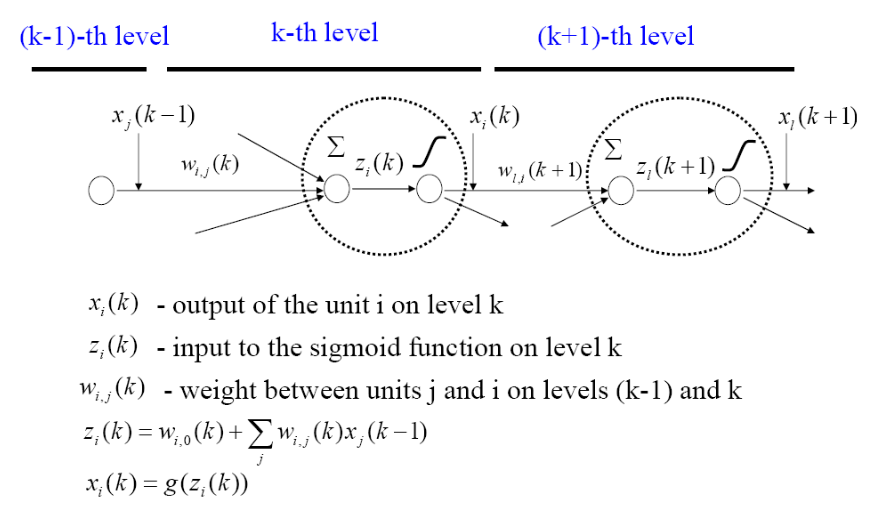
\includegraphics[scale=0.26]{figs/layer.png}
\end{center}

By making this decision, instead of having to think about the values $z$, $w$ and so on with respect to \textit{multiple} layers in the overall network, I could isolate the operations for each individual layer before building them up into a larger network. So, each Layer object holds the following attributes:
\begin{itemize}
	\item [] 1. \texttt{self.weights}: A weight matrix corresponding to $w_{i,j}^{(k)}$ in the figure above.
	\item [] 2. \texttt{self.nodes}: A integer holding the number of nodes in the layer corresponding to $i$ in the figure.
	\item [] 3. \texttt{self.activation}: A pointer to the activation function corresponding to $g()$. The options offered in this implementation are \textit{tanh}, \textit{sigmoid}, and \textit{ReLU} (\textit{softmax}, as well, but this is only recommended for use in the output layer).
	\item [] 4. \texttt{self.activation\_deriv}: A pointer to a function which calculates the \textbf{derivative} of the activation function, which is used during the backpropogation step.
	\item [] 5. \texttt{self.z}: A list containing the result of the weighted sum calculation of the inputs from the previous layer and the weights, for each node, corresponding to $z_i^{(k)}$.
	\item [] 6. \texttt{self.activations}: A list containing the node activation values, also referred to as the output for each node, corresponding to $x_i^{(k)}$. Another way to think about these values is that they are the weighted sum result in \texttt{self.z}, passed through the layer's activation function.
	\item [] 7.  \texttt{self.delta}: A list containing the delta/error values for each node, computed during the backpropagation step, referred to by $\delta_i^{(k)}$ in the course lecture materials.
\end{itemize}

Of these elements, \texttt{self.nodes}, \texttt{self.activation}, and \texttt{self.activation\_deriv} are static throughout the training process, and the other elements are updated during each backpropagation steps. These elements are all that are necessary for all of the hidden layer operations (other than, of course, the input from other layers/training features). 

Now, on to the actual operations themselves, the crucial components of the neural network prediction and backpropagation training algorithms. We know that the weights must be initialized prior to any network training, so I included a function for this purpose, which takes in the number of inputs from the preceding layer (we'll call it $j$ here, to be consistent with the figure above) and generates an $i$ $\times$ $j$ matrix of random floats. Initially, I chose the weights randomly selected from a uniform distribution ranging from -0.5 to 0.5. I'd like to say that I had a very particular reason for choosing this particular range for initializing the weights, but unfortunately I was, for the most part, drawing on my own intuition, as well as settings from previous homeworks. This is the method that was used for the first three, simple experiments described below, which are primarily proof-of-concept experiments, and these weights worked fine. However, as I will discuss later in the report, the final experiment with a more complex dataset was tricker to train the model successfully on. There are many factors involved, far more than I had time to delve into in the course of this project, but a simple change I could make was thinking a bit more critically about how to initialize the weights, as this can impact the performance of the model significantly.

Unfortunately, the scope of the project did not allow me to dig too deeply into the full mathematical motivations behind the particular weight initialization methods, but the general intuition is that, depending on how the weights are initialized, the repeated matrix multiplications involved can result in layer activations either "exploding" -- get so large that the computer can no longer hold the values, or "vanishing" -- essentially the reverse. These phenomenon can, understandably, have detrimental effects on the convergence of the algorithm. Although it seems that these issues come about much more often in models with a very large number of layers, I thought that choosing a less intuition-based initialization approach may produce better results for my more complex dataset. In the research I did have time to do on the matter, I discovered two different strategies for initialization:

\begin{itemize}
	\item [] Xavier method: This method is suggested for weight initialization on layers with \textit{sigmoid} or \textit{tanh} activation functions, and involves setting the weights to be drawn from a uniform distribution ranging from $\pm\frac{\sqrt{6}}{\sqrt{j + i}}$. 
	\item [] Kaiming method: This method is recommended for layers with \textit{ReLU} activation functions, and involves first initializing the weight matrix to values from a standard normal distribution  ($mu=0$, $\sigma=1$), and then multiply each value by $\frac{\sqrt{2}}{\sqrt{j}}$. The bias column is set to all zeros.
\end{itemize}

I'll discuss how these perform later in the report, but I did modify the Layer class's weight initialization  function \texttt{initialize\_weights} to use the recommended method for the activation function it was set to, in hopes that the model would perform better on the complex data. Please see citation \#1 for the source material from which I learned much of the information related to weight initialization!

Now, the next important operation a layer must be able to do is calculate the forward-pass values, which, as we all know quite well by now, is performed using the following formula, where the $x$ values correspond to the input from the previous layer (note: I do integrate the bias into the feature matrix, by adding an initial column of ones, so the bias does not need to be explicitly handled here):

$$z_i = \sum_{j}^{} w_{i,j}x_j$$ 

 This is a very simple process in the code, taking as input the output from the previous layer, and then computing the weighted sum for each node by performing matrix multiplication using the current layer's weights (\texttt{self.weights}) by the input values. These values are saved into \texttt{self.z} for use in the backpropagation operation. The corresponding symbolic formula is as follows, with $h()$ representing the activation function:
 
 $$a_i = h(z_i)$$
 
 After computing the values for \texttt{self.z}, these values are passed into the activation function. Since the pointer to the activation function is set when the layer is initialized, the code only needs to pass the $z$ values into \texttt{self.activation()}, and the correct activation function will be used to compute \texttt{self.activations}. This method of saving the activation function itself as a data member for the Layer object allows the code to be written in a simple, flexible, and straight-forward fashion, despite allowing for multiple activation function options. 
 
 Perhaps the most important operation a layer must do is compute the error/delta values using backpropagation. I made an important design decision here -- that I would simplify this function by assuming these Layer objects, when created by a user and added to a network, would correspond to hidden layers, and that the larger NeuralNetwork class would handle creating the final output layer and performing the backpropagation step for that layer. So, the Layer class could stick to calculating the error values for hidden layers, simplifying this function significantly. 
 
 I'll take a moment to digress from the more practical implementation discussion to give a brief overview of the backpropagation process. As we well know, to perform weight updates that will reduce the error of the overall network using gradient descent, we must calculate the gradient of the cost function $E$ on the current set of inputs ($x_n$)  and current weights, which gives us the direction of the steepest increase, and subsequently update/improve the weights by \textit{subtracting} the gradient values, so that we minimize the output of the cost function. So, we must determine the derivative of the cost function with respect to each individual weight, in order to update the weights correctly. 
 
 Although this content can be found across the web, as well as in our textbook, I'd like to quickly recap the derivation as it relates to my implementation. Please keep in mind, the derivation in the text book orders the layers using the subscripts $i$, $j$, $k$ to refer to the previous, current, and next layer respectively, whereas the notation in the lecture, which I am using in this report uses $j$, $i$, $l$. So, put the process into mathematical terms, we must find $\frac{\partial E_n}{\partial w_{i,j}}$ for each $i$,$j$ pair across all layers. Using the chain rule, we can break down the derivative into the following two partial derivatives, with respect to the layer activations:
 
 $$\frac{\partial E_n}{\partial w_{i,j}} = \frac{\partial E_n}{\partial z_{i}} \frac{\partial z_{i}}{\partial  w_{i,j}}$$
 
 Then, given that $z_i = \sum_{j}^{} w_{i,j}x_j$, where $x_j$ is the output of the previous layer, thus equivalent to $a_j$, we know that:
  $$\frac{\partial z_{i}}{\partial  w_{i,j}} = a_j$$
  
  The other partial derivative, $\frac{\partial E_n}{\partial z_{i}}$, is typically denoted using the symbol $\delta_i$. It's quite straightforward to calculate this value, once the derivative is taken. For the sake of brevity, I will not include derivations for each cost function, but this is of little consequence, since as long as the cost function being used is the canonical link function for the output activation function, we get the same basic formula (where $y_n$ refers to the true label/value for the current example/input $x_n$, and $a_{final}$ to the final output from the forward pass through the network, essentially, the predicted label/value for the input, given the current weights):
  
  $$\delta_{final} = y_n - a_{final} $$
 
 The final activation/cost function pairs, along with the typical use-case, for which this is valid are identity activation with sum-of-squares error for regression, sigmoid activation with binary cross-entropy error for binary classification, and softmax activation with multiclass cross-entropy error for multiclass classification. As this section is getting quite long, I will not include these formulas...but they are all present in the \texttt{utils.py} module!
 
 Now that we have a formula for the delta/error values for the final layer, we can derive the same for the hidden layers, again using the chain rule for partial derivatives, along with the definition of $z_i$ and knowing we can substitute $\delta_*$ for $\frac{\partial E_n}{\partial z_{*}}$:
 
 $$\delta_i = \frac{\partial E_n}{\partial z_{i}} = \sum_{l} \frac{\partial E_n}{\partial z_{l}} \frac{\partial z_l}{\partial z_{i}} = h'(x_i)\sum w_{l,i} \delta_l$$
 
 Alright! After all that, we have the formula that is used in the Layer class's backpropagation formula. Once again, since we are assuming this will only be called for hidden layers, we need not concern ourselves with the formula for computing the final layer's delta values. Additionally, since we are passing in the activation function's derivative ($h'()$) as a pointer to a function, we can just use \texttt{self.activation()} to calculate the result of this derivative on the $z$ values. So, using this formula, and taking as input the next layer's delta and weight values, the backpropogation function calculates the layer's \texttt{self.delta} values.
 
The final operation for the Layer class is the weight update. This process is quite simple, given the derivation above, we know that the derivative with respect to each weight (i,e., the gradient), is calculated using the following formula:

$$\frac{\partial E_n}{\partial w_{i,j}} = \delta_i a_j $$

So the weight update function takes as input the previous layer's activations, calculates the outer product of the current layer's delta values with the values input, resulting in the derivative for each weight. These values are subsequently multiplied by the learning rate (which will be discussed shortly), and subtracted from the current weight values.

Setting up the Layer class was perhaps the trickiest part of this project, despite being a relatively small set of short functions. However, having these methods in place made building the NeuralNetwork class quite straight-forward, which I'll wrap up this section by discussing. The NeuralNetwork class is used to build a NeuralNetwork with a custom architecture, and is initialized by setting a number of parameters:

\begin{itemize}
	\item [] \texttt{self.input\_nodes}: The number of input nodes, or number of training data's features/attributes.
	\item []  \texttt{self.output\_nodes}: The number of output nodes. If multiclass, this is the number of classes, if regression or binary classification, this should be set to 1.
	\item [] \texttt{self.output\_activation}: A pointer to the output activation function corresponding to the type of problem (regression $\longrightarrow$ identity, binary classification $\longrightarrow$ sigmoid, multiclass classification $\longrightarrow$ softmax).
	\item [] \texttt{self.output\_deriv} A pointer to the function of the derivative of the output function. This is a relic of an initial version of the program, before I realized this would not be necessary. 
	\item [] \texttt{self.objective\_fcn} A pointer to the objective/cost function for the problem being considered (regression $\longrightarrow$ sum-of-squared, binary classification $\longrightarrow$ binary crossentropy, multiclass classification $\longrightarrow$ multiclass crossentropy)
	\item []  \texttt{self.learning\_rate}: The learning rate by which gradient updates are multiplied prior to applying to weights.
\end{itemize}

In retrospect, it may have been easier from the user's perspective to have them just pass in the name of the type of problem they will be using the network to solve (regression, etc), and set them internally, but alas, that is a small issue so I did not address it here. The initialization function also generates a Layer object for the output layer, using the objective function passed in by the user. 

It's worth noting, that if the user does not add any hidden layers to the network, it can still be used. In this case, it is simply a logistic/linear regression model, but is still useful for linearly separable data! On that note, the NeuralNetwork also has an \texttt{add\_layer} function, where the user can pass in a Layer object, and it is appended to the NeuralNetwork's \texttt{self.layers} list, which is used during the fitting and predicting functions.

After the user has added their desired layers, they can call the \texttt{fit()} method. The user can pass in the desired number of epochs to train the model on, and can decide if they would like to use early stopping as a regularization method by passing in a validation data set. If early stopping is desired, the user must decide how many epochs in a row they will allow the validation error to increase before freezing the model weights and ending the fitting process. This ensures that the model does not overfit to the training data, and the fitted weights will allow generalization to new data.

This \texttt{fit()} method consists of perhaps the most code in terms of lines, but is not terrible complicated in that it generally follows the online gradient descent algorithm provided in class. The first step involves adding the bias feature to the training feature matrix, as an initial column of ones. Next, it initializes the weights for all layers, which simply involves iterating through each layer, calling the Layer method \texttt{initialize\_weights}, passing in number of nodes from the previous layer (or in the case of the first layer, the number of input features). 

After these steps have been taken, the actual learning algorithm begins. As mentioned, I decided to stay simple for this project and only give the option for stochastic/online gradient descent. Although it wouldn't be difficult to accumulate the errors over an entire epoch or mini-batch, and then perform the weight update, adding this as an option would have ballooned my experiment analyses to extreme sizes. As I understand it, although batch processing does operate on a static cost function, resulting in a smooth descent, it is not ideal for complex datasets that may have non-convex cost functions. Stochastic gradient descent is a better choice for these complex datasets, as they descend on the cost function for each individual sample, which adds an element of noise to the overall process, potentially allowing the algorithm to overcome traps of local minima on the way to finding the global minimum. However, stochastic gradient descent may be more computationally taxing, since each sample must be iterated over individually, disallowing some efficient tensor operations that are available in Python. All in all, from the research I've done, as well as the information on this matter in the textbook, I've gleaned that online gradient descent is often a better choice than batch processing, and mini-batch processing is superior to both, as it combines the best of both options.

So, to implement stochastic gradient descent, I loop over the following process for the user's desired number of epochs:

\begin{itemize}
	\item [] 1. Randomly select an example from the training set, without replacement. If no more samples, end epoch.
	\item [] 2. Calculate $f(x_i, w)$, or the output/prediction of the model on that example's features by performing a forward pass through all layers. The first layer takes in $x_i$ as input to the \texttt{forward\_pass()} Layer method described above, and each subsequent layer output is passed into the next layer's \texttt{forward\_pass()} method. The error is then calculated using the output of the final layer and the user-selected objective function, in order to report on the epoch average error.
	\item [] 3. Calculate the $\delta$ values for the final layer using the formula described above.
	\item [] 4. For each layer, going backwards from the previous layer, call the aforementioned Layer \texttt{backpropagation()} method, passing in the previous layer's $\delta$ values and weight matrix.
	\item [] 5. Perform the weight updates for each layer, starting from the front and going to the end, again, using a Layer function; \texttt{weight\_update()}.
	\item [] 6. Continue this process until all examples have been used.
\end{itemize}

After this loop/epoch, the early stopping criteria is tested. That is, the validation data set error is calculated, using the current set of weights. If the validation error is larger than the previous validation error, we add one to the value tracking sequential error increases, and if it is not, we reset that value to zero. If the value tracking increases has hit the maximum the user has passed in, the training process concludes. Otherwise, the training process continues until all epochs have run. 

Finally, if the user desires, the function can print out a plot of the training and validation errors for each epoch, to see the error trajectory over the course of the training process.

The NeuralNetwork class also offers a \texttt{predict()} method, which takes in a test set of features, and uses the current model weights to predict the output, whether a real number for regression, or a vector containing the class that each sample is predicted to belong to. In addition to this function, the class also has an \texttt{evaluate()} method, which allows the user to pass in a set of test features $X$ and corresponding ground truth labels $y$, and computes the mean error over the set, as well as the class accuracy, if applicable.

That concludes the description of my implementation of the flexible neural network framework, and the remainder of the code in the file is related to the individual experiments to validate the framework's functionality, which are described in the remainder of the report.

\end{quote}

\subsection*{Data}
\begin{quote}
\setlength{\parindent}{10ex}
\quad\quad\quad\quad Since the framework was built to be very flexible, to allow for use on a number of different problem/dataset types, I needed to make sure that all possible conditions were exercised and determined to be functioning correctly before deeming the implementation a success. To do this, I decided to perform a number of experiments using standard, toy datasets, one for each type of problem.

To test the framework's ability to solve regression problems, which requires the identity function as the output layer activation function, and sum-of-squared error as the objective function, I decided to use the classic Boston Housing dataset. I opted to use this set, since not only was is easily available through sklearn's datasets module, but also we spent some time evaluating simpler regression models using this data in Homework 2. So, I would have my own baseline of comparison to use, since it's rather tricky to tell just how well a regression model is performing using the error rate (there's no universal metric such as accuracy, that I'm aware of). This dataset is somewhat small, containing 506 examples with 13 features corresponding to various housing attributes, and a single target corresponding to median value.

The second dataset is a simple, classic set often used to benchmark binary regression algorithms; the Wisconson Breast Cancer diagnostic dataset. This, like all of the toy datasets I'm using for this project, is available quickly and easily in sklearn.datasets. The dataset has 569 examples, with 30 diagnostic features pertaining to characteristics of cell nuclei, and a single, binary target -- whether the cell is malignant (0) or benign (1). It is important to note that this dataset is not quite balanced, it has more benign examples than malignant, although the imbalance is not so much that I would expect it to hinder classification. 

The third, and final of the toy datasets is the classic of all classics, the Iris dataset. This dataset consists of 150 examples, each with 4 features reflecting several features of the flowers. There are three possible classes, according to which specific type of iris each example is. This dataset is completely balanced, with 50 examples for each class. The dataset is known to not be linearly separable in all classes, so this is a good candidate to verify that adding non-linearity via multiple layers aids in classification performance.

After ensuring the datasets above result in reasonably well-trained models, I will move on to experiment with a slightly more complex dataset; the Ryerson Audio-Visual Database of Emotional Speech and Song (RAVDESS) dataset. This is a dataset consisting of audio-visual data from twenty-four actors, evenly split across genders, each speaking or singing a short phrase with tone/inflection corresponding to eight different emotions, such as ``happy", ``fearful", and ``sad". I chose to isolate the subset of files with audio data only, and just those speaking the phrase, not singing. Although the dataset description notes that there should be 1440 examples, the version of the dataset I downloaded has only 1428 examples. 

I performed some very simple preprocessing of the files by first removing the silence at the beginning and end of the wav file, using the handy `PyDub'/`audiosegment' Python packages. This process did not perform perfectly, removing 12 files completely, so these files were not used in the experiments, resulting a final set containing 1416 examples. The remaining files were spot-checked, and the silence-removal process worked well for the files checked. The `python-speech-features' package was used to calculate mel-frequency filter bank values, a common method of generating features from audio files, and the resulting frame-wise features were averaged to create one vector of 26 features for each utterance. As mentioned, the dataset consisted of audio samples belonging to one of eight classes, depending on what emotion was being conveyed. The dataset was balanced, for the most part, although there are only half as many examples for the `neutral' class than for all other classes.
\end{quote}

\subsection*{Results}
\begin{quote}
	\setlength{\parindent}{10ex}
	\quad\quad\quad\quad Now, I'll discuss experiments and results for each dataset. Several parameters were held constant across all datasets: train, validation, and test set proportions (20\%, 16\%, and 64\% respectively), inclusion of bias, and scaling of feature data, using sklearn's StandardScaler, which standardizes the data using the Z-score method (scaler is ``fit" using training set data only). When multiple hidden layers are included in the network architecture, all layers have the same activation function, and same number of nodes. Since these simple datasets are more to verify basic functionality, and the the results are not terribly interesting given the simplicity of the data, I limited the conditions tested. Additionally, for the simple datasets, early stopping was not activated, so the network was trained for the full number of epochs specified in the tables below.
	
	All tests were performed using the same random seed, and identical test/train/validation splits for each dataset. This was done to ensure that any differences came from the differing network architectures, not artifacts of weight initialization or particular data points contained in each split.
\end{quote}

\clearpage
\subsubsection*{Boston Housing Dataset: Simple Regression}
\begin{quote}
	\setlength{\parindent}{10ex}
		\quad\quad\quad\quad Below are the results from a number of different test conditions/architectures using the Boston Housing dataset, along with plots showing the test and validation error, per epoch, for each condition. Note that all experiments used the identity function as the final layer activation, and sum-of-squares error for the cost function:

	\begin{table}[h!]
		\centering
		\begin{tabular}{|c|c|c|c|l|c|c|}
			\hline
			\begin{tabular}[c]{@{}c@{}}Activation\\ Function\end{tabular} & Epochs                & \begin{tabular}[c]{@{}c@{}}Learning\\ Rate\end{tabular} & \begin{tabular}[c]{@{}c@{}}Hidden\\ Layers\end{tabular} & \multicolumn{1}{c|}{\begin{tabular}[c]{@{}c@{}}Nodes\\ Per Layer\end{tabular}} & \begin{tabular}[c]{@{}c@{}}Mean Test\\ Error\end{tabular} & \begin{tabular}[c]{@{}c@{}}Test\\ Accuracy\end{tabular} \\ \hline
			&                       &                                                            & 1                                                       & 8                                                                              & 7.80                                                 & \multirow{3}{*}{N/A}                                    \\ \cline{5-6}
			Sigmoid                                                          & 20                    & 0.01                                                       &                                                         & 16                                                                             & 8.44                                                 &                                                         \\ \cline{4-6}
			&                       &                                                            & 2                                                       & 8                                                                              & 9.01                                                 &                                                         \\ \cline{5-6}
			\multicolumn{1}{|l|}{}                                           & \multicolumn{1}{l|}{} & \multicolumn{1}{l|}{}                                      & \multicolumn{1}{l|}{}                                   & 16                                                                             & 5.08                                                 &                                                         \\ \hline
			&                       &                                                            & 1                                                       & 8                                                                              & 7.16                                                 & \multirow{3}{*}{N/A}                                    \\ \cline{5-6}
			ReLU                                                             & 20                    & 0.001                                                      &                                                         & 16                                                                             & 6.26                                                 &                                                         \\ \cline{4-6}
			&                       &                                                            & 2                                                       & 8                                                                              & 7.11                                                 &                                                         \\ \cline{5-6}
			\multicolumn{1}{|l|}{}                                           & \multicolumn{1}{l|}{} & \multicolumn{1}{l|}{}                                      & \multicolumn{1}{l|}{}                                   & 16                                                                             & 7.51                                                 &                                                         \\ \hline
			&                       &                                                            & 1                                                       & 8                                                                              & 11.06                                                & \multirow{3}{*}{N/A}                                    \\ \cline{5-6}
			Tanh                                                             & 20                    & 0.001                                                      &                                                         & 16                                                                             & 10.39                                                &                                                         \\ \cline{4-6}
			&                       &                                                            & 2                                                       & 8                                                                              & 10.97                                                &                                                         \\ \cline{5-6}
			\multicolumn{1}{|l|}{}                                           & \multicolumn{1}{l|}{} & \multicolumn{1}{l|}{}                                      & \multicolumn{1}{l|}{}                                   & 16                                                                             & 11.16                                                &                                                         \\ \hline
		\end{tabular}
	\end{table}
	\setlength{\parindent}{10ex}
	 \begin{figure}[h]
		\centering
		\begin{subfigure}[h]{0.23\textwidth}
			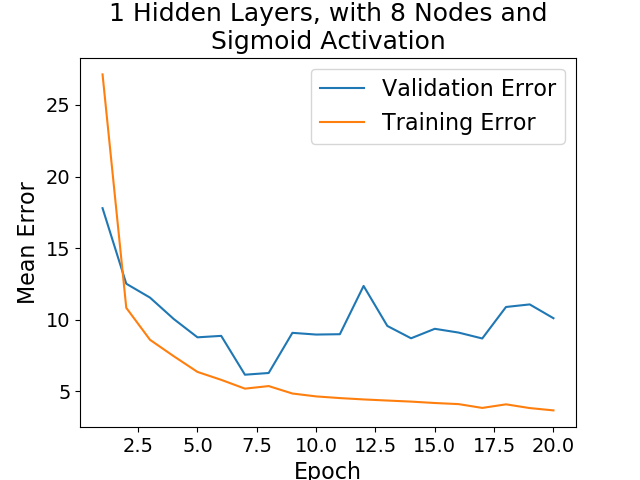
\includegraphics[width=\textwidth]{figs/Boston_Housing_Regression_1_Hidden_Layers_with_8_Nodes_and_Sigmoid_Activation.png}
		\end{subfigure}
		%
		\begin{subfigure}[h]{0.23\textwidth}
			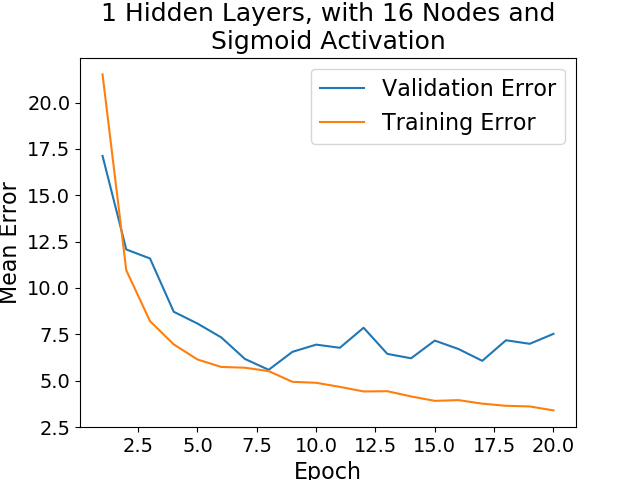
\includegraphics[width=\textwidth]{figs/Boston_Housing_Regression_1_Hidden_Layers_with_16_Nodes_and_Sigmoid_Activation.png}
		\end{subfigure}
			%
		\begin{subfigure}[h]{0.23\textwidth}
		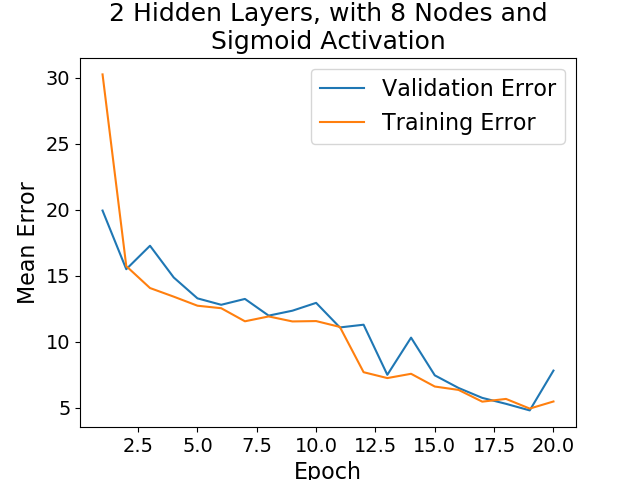
\includegraphics[width=\textwidth]{figs/Boston_Housing_Regression_2_Hidden_Layers_with_8_Nodes_and_Sigmoid_Activation.png}
		\end{subfigure}
		%
		\begin{subfigure}[h]{0.23\textwidth}
		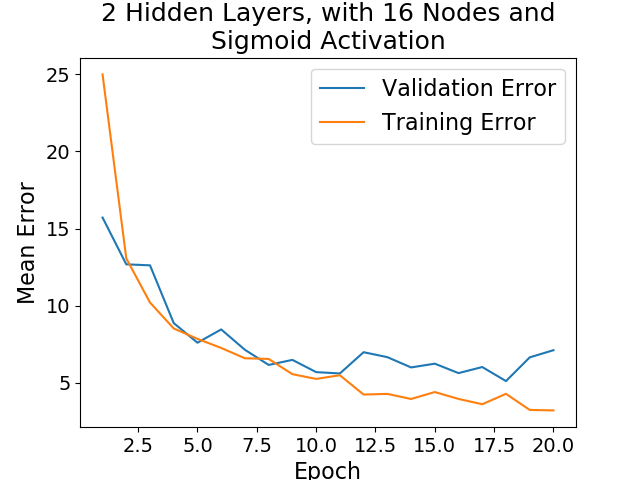
\includegraphics[width=\textwidth]{figs/Boston_Housing_Regression_2_Hidden_Layers_with_16_Nodes_and_Sigmoid_Activation.png}
		\end{subfigure}
	\end{figure}	
	 \begin{figure}[h]
	\centering
	\begin{subfigure}[h]{0.23\textwidth}
		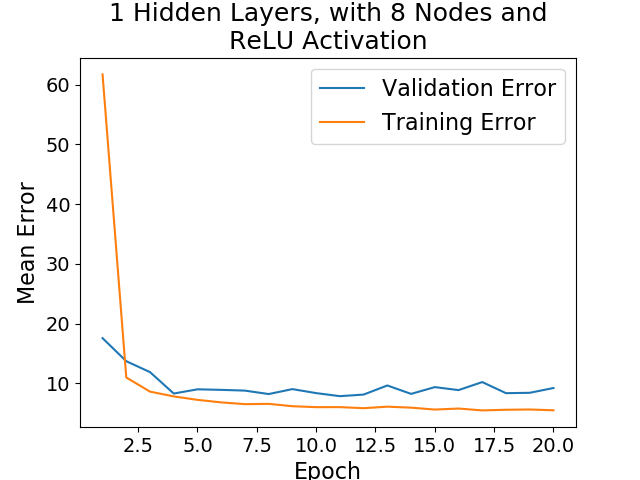
\includegraphics[width=\textwidth]{figs/Boston_Housing_Regression_1_Hidden_Layers_with_8_Nodes_and_ReLU_Activation.png}
	\end{subfigure}
	%
	\begin{subfigure}[h]{0.23\textwidth}
		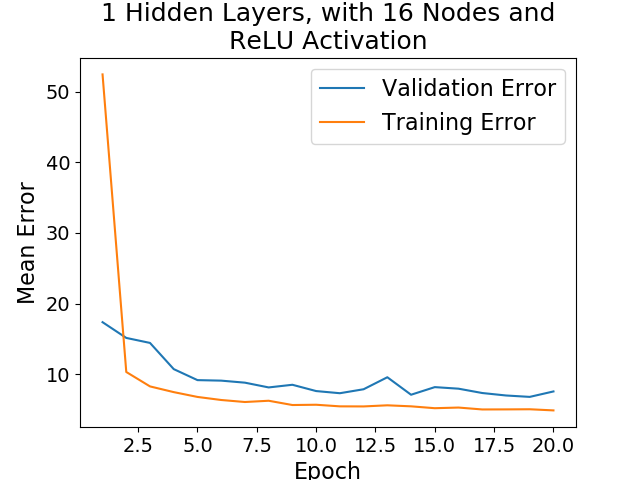
\includegraphics[width=\textwidth]{figs/Boston_Housing_Regression_1_Hidden_Layers_with_16_Nodes_and_ReLU_Activation.png}
	\end{subfigure}
	%
	\begin{subfigure}[h]{0.23\textwidth}
		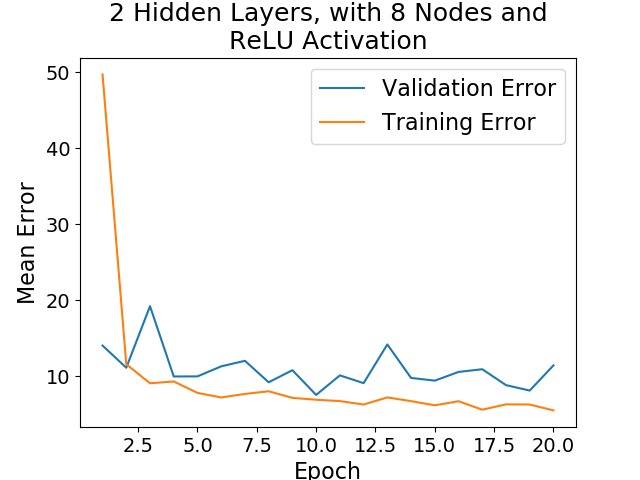
\includegraphics[width=\textwidth]{figs/Boston_Housing_Regression_2_Hidden_Layers_with_8_Nodes_and_ReLU_Activation.png}
	\end{subfigure}
	%
	\begin{subfigure}[h]{0.23\textwidth}
		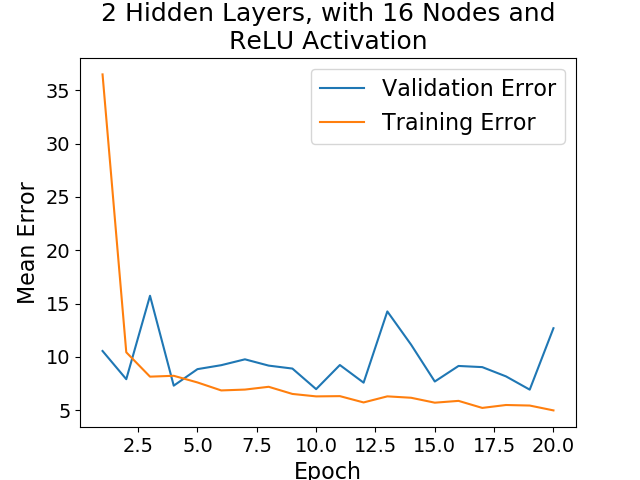
\includegraphics[width=\textwidth]{figs/Boston_Housing_Regression_2_Hidden_Layers_with_16_Nodes_and_ReLU_Activation.png}
	\end{subfigure}
\end{figure}	
	 \begin{figure}[h!]
	\centering
	\begin{subfigure}[h]{0.23\textwidth}
		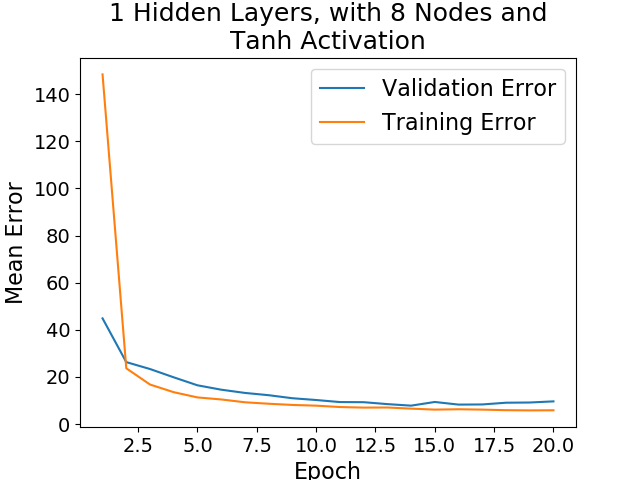
\includegraphics[width=\textwidth]{figs/Boston_Housing_Regression_1_Hidden_Layers_with_8_Nodes_and_Tanh_Activation.png}
	\end{subfigure}
	%
	\begin{subfigure}[h]{0.23\textwidth}
		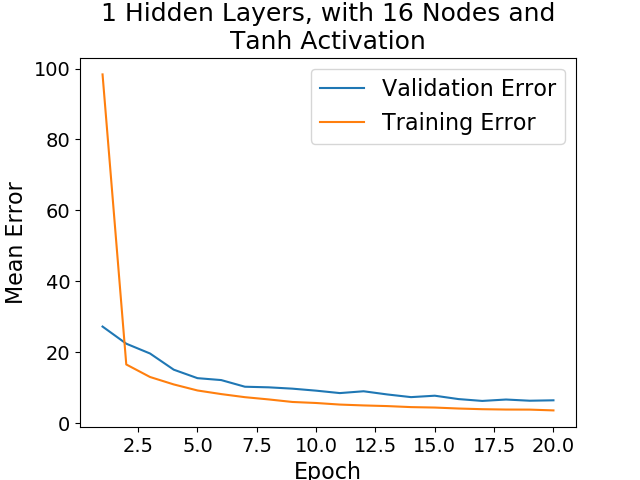
\includegraphics[width=\textwidth]{figs/Boston_Housing_Regression_1_Hidden_Layers_with_16_Nodes_and_Tanh_Activation.png}
	\end{subfigure}
	%
	\begin{subfigure}[h]{0.23\textwidth}
		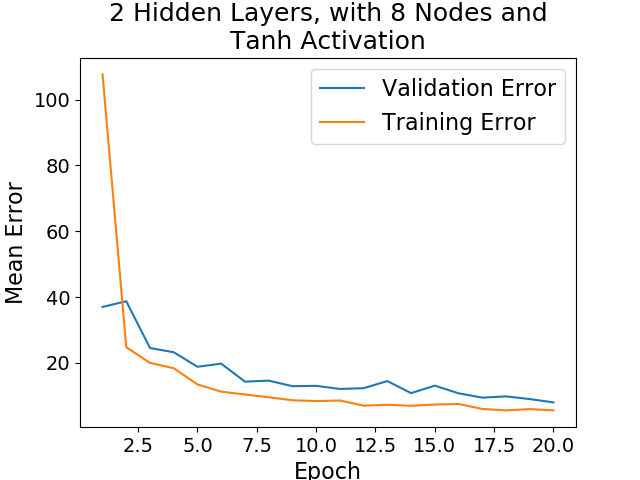
\includegraphics[width=\textwidth]{figs/Boston_Housing_Regression_2_Hidden_Layers_with_8_Nodes_and_Tanh_Activation.png}
	\end{subfigure}
	%
	\begin{subfigure}[h]{0.23\textwidth}
		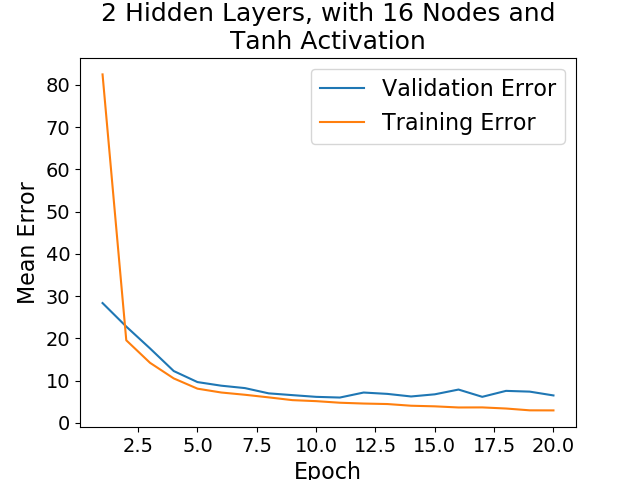
\includegraphics[width=\textwidth]{figs/Boston_Housing_Regression_2_Hidden_Layers_with_16_Nodes_and_Tanh_Activation.png}
	\end{subfigure}
\end{figure}


	 As mentioned, this is a simple toy regression dataset, often used in a teaching concept to demonstrate the functionality of various learning algorithms. While the neural network model is, perhaps, slightly ``overkill" for dealing with this simple dataset, I wanted to evaluate the network performance for a regression task on a dataset for which I knew the model should achieve low error. So, as a baseline, I considered the mean squared error achieved in Homework 2, using linear regression. On this homework assignment, the online gradient descent algorithm for linear regression achieved $\approx$ 66 MSE. 
	 
	 It is important to note that these error rates were calculated using mean squared error, and in this project, I am using mean SSE to calculate the error, which would need to be multiplied by two to be equivalent to MSE. However, even if we multiply all of the MSE values in the table above by two, we have still achieved better performance for this dataset by incorporating non-linearity through additional layers with non-linear activation functions. 
	 
	 As a sanity check, I also ran the neural network model \textit{without} any hidden layers, which would be equivalent to linear regression, for the best possible comparison, considering the test-train split in Homework 2 was not the same one used for the trials above, and the learning rate was not the same as used in this context. This architecture achieved a test mean error of $\approx$ 17.8, which, as expected, is a fair bit higher than any of the errors achieved with the more complex architectures, implying that adding non-linearity to the architecture, regardless of the particular activation function chosen, results in a better performing model.
	 
	 We can make a number of other interesting observations based on the table and plots above. The first piece of information that pops out at me if that the best-performing architecture is the model with two hidden layers with 16 nodes each, and sigmoid activation. I was rather surprised by this, since this was the most complex architecture in the experiment, and I'd assumed that this dataset may be prone to overfitting since it is relatively simplistic. For that reason, I'd expected the simpler architectures to perform better as far as how the generalize to new data. I did find that increasing the layers beyond two does result in poorer performance, so perhaps two layers with 16 nodes is the sweet spot for this dataset, at least for the sigmoid activation function.
	 
	 The tanh function is supposedly a better choice, over sigmoid, for the activation function, as it has many of the same attributes but fewer drawbacks, but it performed about equally on average with sigmoid for this particular dataset. These functions are similar, in that both restrict the size of the output of the neuron (sigmoid, between 0-1, tanh between -1 and 1). This feature prevents the ``exploding"  issue mentioned in the context of weight-setting in the methods section, but this is limiting as well. Due to these restrictions, when the input gets quite large or small, the neuronal output will be the same, and the predictions will not change with changes in the gradient. This is referred to as the ``vanishing gradient" problem (see citation \#3), and can understandably cause issues in training. One difference worth noting, however, is that the trajectory of the error functions are quite a bit smoother for the tanh trials than for the sigmoid trials, and the weights appear to generalize to the validation set quite a bit better, with fewer fluctuations.
	 
	 ReLU performed the worst out of all of the activation functions, which again, was somewhat surprising, since this is typically considered the ``best" activation function for a neural network, out of the three choices in this implementation. It is known to result in quick convergence, which we can see in the plots above that it does, for the training set. However, perhaps due to this quick convergence, the model is overfitting, resulting in a very erratic validation error trajectory, and poorer test error. I do want to note that I did encounter the ``exploding" issue when running tests using the ReLU activation with this dataset. This was slightly surprising, as I would expect this to be an issue more-so in neural network architectures with many hidden layers, as the problem is to be exacerbated by many matrix multiplication operations in a row. I was able to offset this error by decreasing the learning rate, but in the future, I'd like to take more time to research this problem, and find better, more structured methods of solving the problem. 
	 
	 I'm sure there are more analyses and more tweaking that could be done to improve the architecture for this dataset, and if I had more time to invest in it, I think I would start by trying different architectures and learning rates using the tanh activation function. But, the point of running this experiment was to ensure that the framework could successfully fit a regression problem by minimizing the error over a training set, and fortunately, it does!
	 
	 
	 
\end{quote}

\subsubsection*{Breast Cancer Diagnostic Dataset: Simple Binary Classification}
\begin{quote}
		\setlength{\parindent}{10ex}
	\quad\quad\quad\quad Below are the trials from the second experiment, again using a simple, toy dataset, but in this case for binary classification. All trials use a sigmoid output activation function, and a binary cross-entropy cost function:
	
	\begin{table}[h]
		\centering
		\begin{tabular}{|c|c|c|c|l|c|c|}
			\hline
			\begin{tabular}[c]{@{}c@{}}Activation\\ Function\end{tabular} & Epochs                & \begin{tabular}[c]{@{}c@{}}Learning\\ Rate\end{tabular} & \begin{tabular}[c]{@{}c@{}}Hidden\\ Layers\end{tabular} & \multicolumn{1}{c|}{\begin{tabular}[c]{@{}c@{}}Nodes\\ Per Layer\end{tabular}} & \begin{tabular}[c]{@{}c@{}}Mean Test\\ Error\end{tabular} & \begin{tabular}[c]{@{}c@{}}Test\\ Accuracy\end{tabular} \\ \hline
			&                       &   & 1  & 8      & 0.0839              & 96.7\%                                                   \\ \cline{5-7} 
			Sigmoid  & 20                    & 0.01                                                    &                                                         & 16                                                                             & 0.0797                                                    & 95.6\%                                                   \\ \cline{4-7} 
			&                       &                                                         & 2                                                       & 8                                                                              & 0.0868                                                    & 97.8\%                                                   \\ \cline{5-7} 
			\multicolumn{1}{|l|}{}                                        & \multicolumn{1}{l|}{} & \multicolumn{1}{l|}{}                                   & \multicolumn{1}{l|}{}                                   & 16                                                                             & 0.0837                                                    & 96.7\%                                                   \\ \hline
			&                       &                                                         & 1                                                       & 8                                                                              & 0.2094                                                    & 94.5\%                                                   \\ \cline{5-7} 
			ReLU                                                          & 20                    & 0.001                                                   &                                                         & 16                                                                             & 0.0941                                                    & 96.7\%                                                   \\ \cline{4-7} 
			&                       &                                                         & 2                                                       & 8                                                                              & 0.1869                                                    & 96.7\%                                                   \\ \cline{5-7} 
			\multicolumn{1}{|l|}{}                                        & \multicolumn{1}{l|}{} & \multicolumn{1}{l|}{}                                   & \multicolumn{1}{l|}{}                                   & 16                                                                             & 0.1586                                                    & 93.4\%                                                   \\ \hline
			&                       &                                                         & 1                                                       & 8                                                                              & 0.1192                                                    & 95.6\%                                                   \\ \cline{5-7} 
			Tanh                                                          & 20                    & 0.001                                                   &                                                         & 16                                                                             & 0.0947                                                    & 97.8\%                                                   \\ \cline{4-7} 
			&                       &                                                         & 2                                                       & 8                                                                              & 0.1020                                                    & 95.6\%                                                   \\ \cline{5-7} 
			\multicolumn{1}{|l|}{}                                        & \multicolumn{1}{l|}{} & \multicolumn{1}{l|}{}                                   & \multicolumn{1}{l|}{}                                   & 16                                                                             & 0.0822                                                    & 96.7\%                                                   \\ \hline
		\end{tabular}
	\end{table}
\setlength{\parindent}{10ex}
\begin{figure}[h!]
\centering
\begin{subfigure}[h]{0.23\textwidth}
	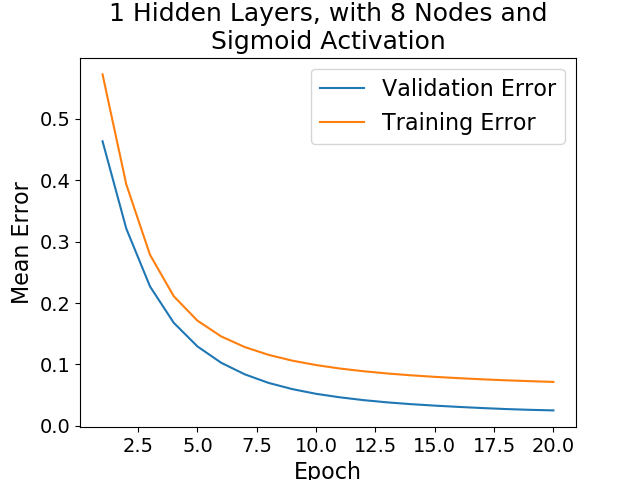
\includegraphics[width=\textwidth]{figs/Cancer_Binary_Classification_1_Hidden_Layers_with_8_Nodes_and_Sigmoid_Activation.png}
\end{subfigure}
%
\begin{subfigure}[h]{0.23\textwidth}
	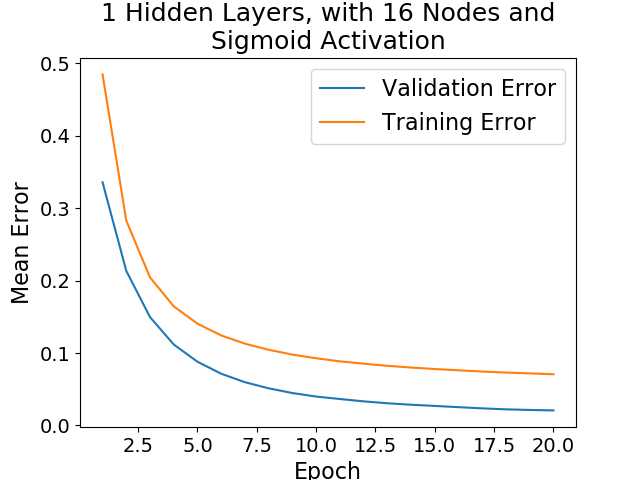
\includegraphics[width=\textwidth]{figs/Cancer_Binary_Classification_1_Hidden_Layers_with_16_Nodes_and_Sigmoid_Activation.png}
\end{subfigure}
%
\begin{subfigure}[h]{0.23\textwidth}
	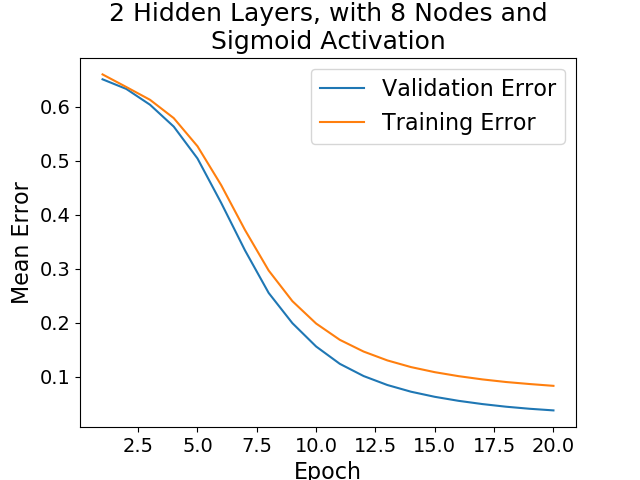
\includegraphics[width=\textwidth]{figs/Cancer_Binary_Classification_2_Hidden_Layers_with_8_Nodes_and_Sigmoid_Activation.png}
\end{subfigure}
%
\begin{subfigure}[h]{0.23\textwidth}
	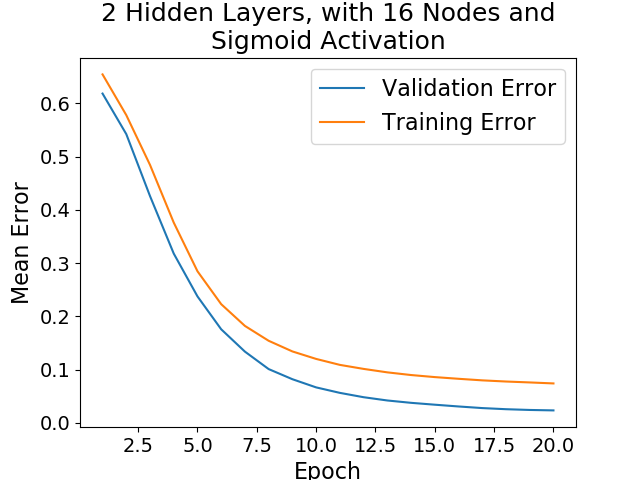
\includegraphics[width=\textwidth]{figs/Cancer_Binary_Classification_2_Hidden_Layers_with_16_Nodes_and_Sigmoid_Activation.png}
\end{subfigure}
\end{figure}	
\begin{figure}[h]
\centering
\begin{subfigure}[h]{0.23\textwidth}
	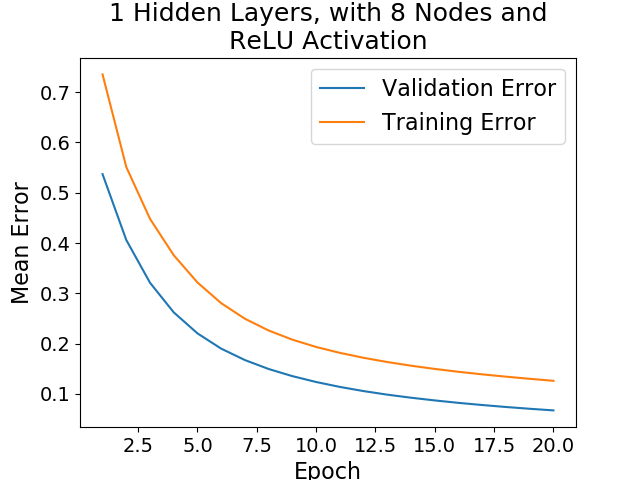
\includegraphics[width=\textwidth]{figs/Cancer_Binary_Classification_1_Hidden_Layers_with_8_Nodes_and_ReLU_Activation.png}
\end{subfigure}
%
\begin{subfigure}[h]{0.23\textwidth}
	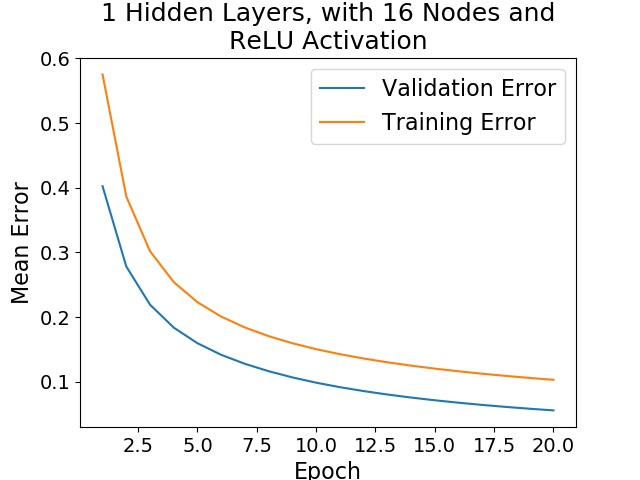
\includegraphics[width=\textwidth]{figs/Cancer_Binary_Classification_1_Hidden_Layers_with_16_Nodes_and_ReLU_Activation.png}
\end{subfigure}
%
\begin{subfigure}[h]{0.23\textwidth}
	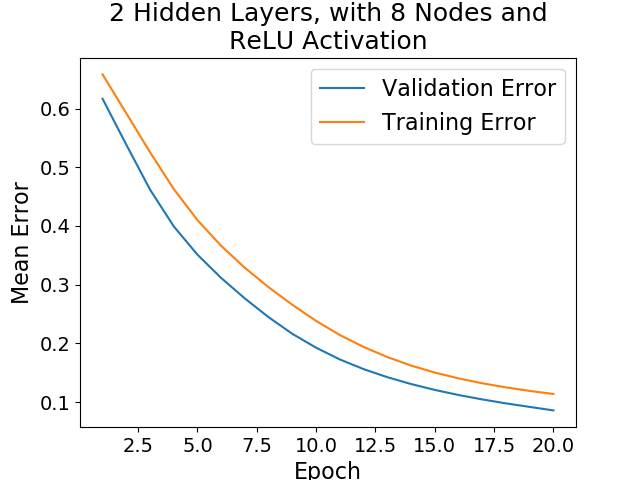
\includegraphics[width=\textwidth]{figs/Cancer_Binary_Classification_2_Hidden_Layers_with_8_Nodes_and_ReLU_Activation.png}
\end{subfigure}
%
\begin{subfigure}[h]{0.23\textwidth}
	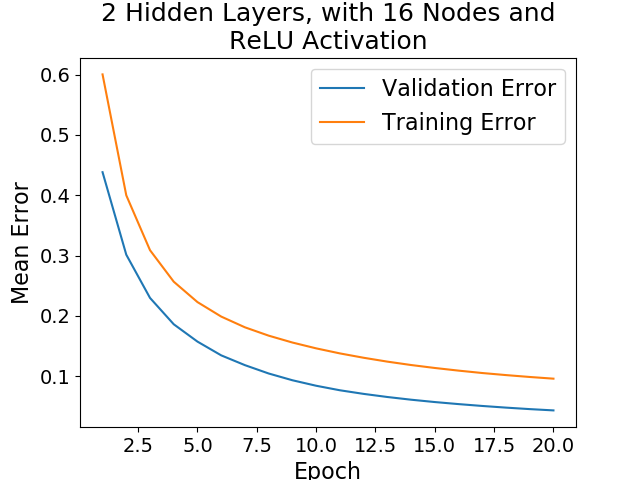
\includegraphics[width=\textwidth]{figs/Cancer_Binary_Classification_2_Hidden_Layers_with_16_Nodes_and_ReLU_Activation.png}
\end{subfigure}
\end{figure}	
\begin{figure}[h!]
\centering
\begin{subfigure}[h]{0.23\textwidth}
	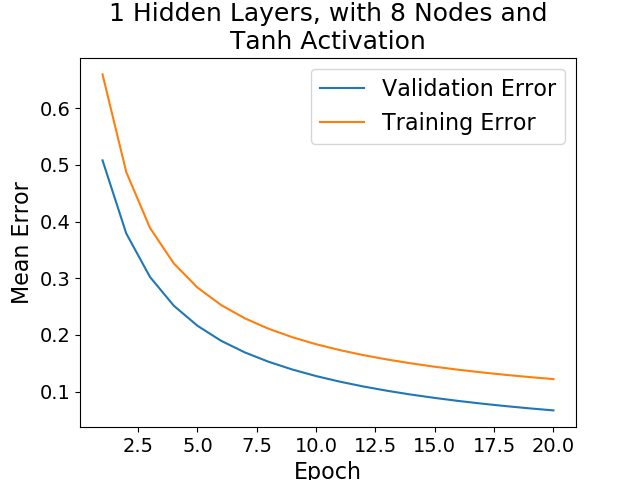
\includegraphics[width=\textwidth]{figs/Cancer_Binary_Classification_1_Hidden_Layers_with_8_Nodes_and_Tanh_Activation.png}
\end{subfigure}
%
\begin{subfigure}[h]{0.23\textwidth}
	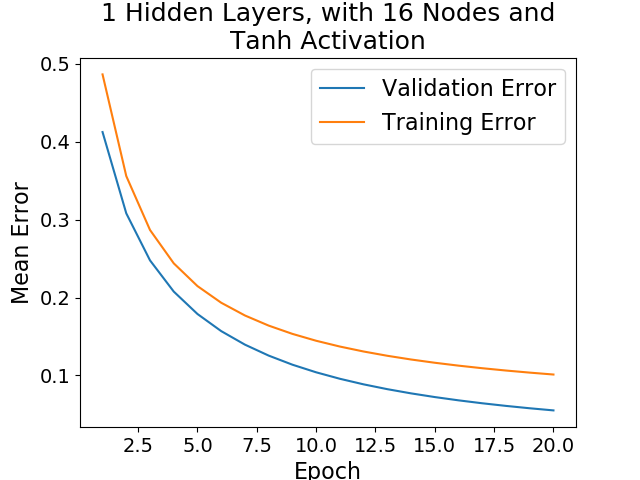
\includegraphics[width=\textwidth]{figs/Cancer_Binary_Classification_1_Hidden_Layers_with_16_Nodes_and_Tanh_Activation.png}
\end{subfigure}
%
\begin{subfigure}[h]{0.23\textwidth}
	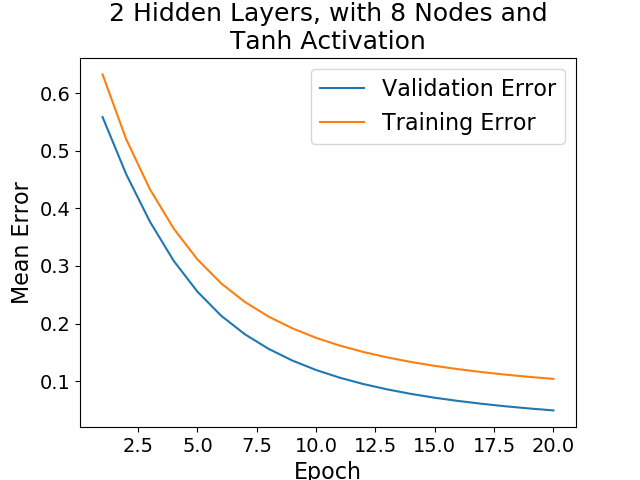
\includegraphics[width=\textwidth]{figs/Cancer_Binary_Classification_2_Hidden_Layers_with_8_Nodes_and_Tanh_Activation.png}
\end{subfigure}
%
\begin{subfigure}[h]{0.23\textwidth}
	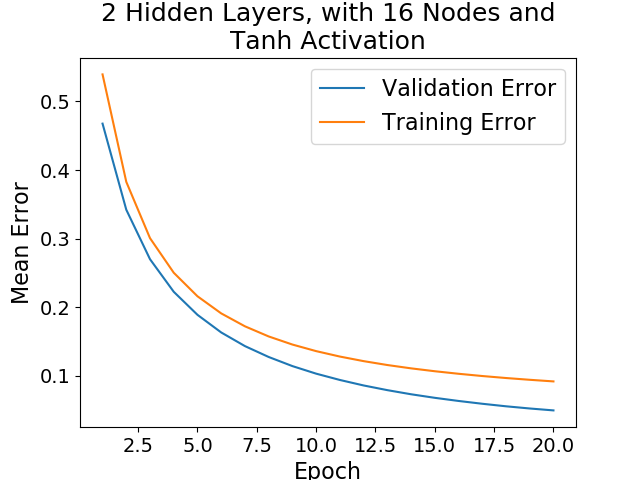
\includegraphics[width=\textwidth]{figs/Cancer_Binary_Classification_2_Hidden_Layers_with_16_Nodes_and_Tanh_Activation.png}
\end{subfigure}
\end{figure}
	We can certainly see from the results above that the model does perform as expected on a binary classification task. I'll keep this discussion brief, as for the most part, the models perform equally well regardless of architecture or activation functions used (with sigmoid performing slightly better than tanh, which performs slightly better than ReLU).
	
	It is, I think, important to compare how well the architectures with hidden layers compare to an architecture without a hidden layer, essentially, a logistic regression model. Training a model with this particular architecture on this dataset resulted in a mean test error of $\approx$ 0.11, and an accuracy of 96.7\%. This result is on par with most of the results from the more complex models, which leads me to believe that this dataset is more-or-less linearly separable. I quickly ran sklearn's PCA algorithm and plotted the first two primary components, to get the following plot:
	
	\begin{center}
		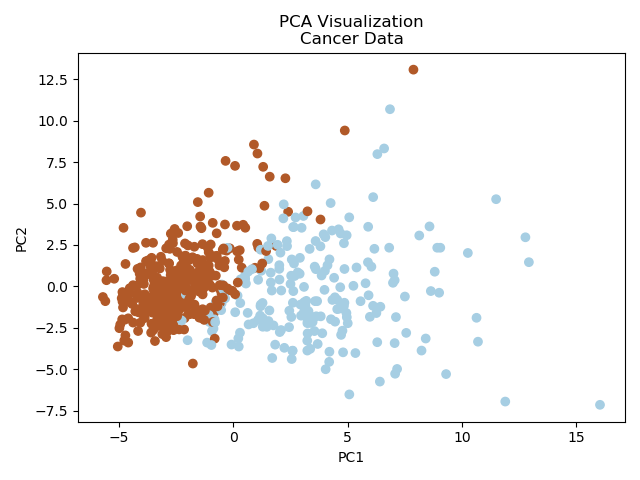
\includegraphics[scale=0.3]{figs/cancer_PCA.png}
	\end{center}
	
	We can see that for at least the two components which explain most of the variance (PC1: 45\%, PC2: 18\%), the dataset does look as though it is almost linearly separable, with a small amount of overlap. So, using a non-linear, multi-layer neural network is not necessary to create a model that can perform well classifying this well-behaved dataset. 
	
	But, again, the motivation behind running this experiment was to ensure that the framework can perform correctly on binary classification, and this has indeed been confirmed!
	
\end{quote}

\subsubsection*{Iris Dataset: Simple Multiclass Classification}
\begin{quote}
			\setlength{\parindent}{10ex}
	\quad\quad\quad\quad The final validation experiment using a toy dataset is below, evaluating the framework's functionality on a multiclass classification problem, specifically the infamous iris dataset. For all trials, the output activation is softmax, and the cost function is multiclass crossentropy:
	
	\begin{table}[h]
		\centering
		\begin{tabular}{|c|c|c|c|l|c|c|}
			\hline
			\begin{tabular}[c]{@{}c@{}}Activation\\ Function\end{tabular} & Epochs                & \begin{tabular}[c]{@{}c@{}}Learning\\ Rate\end{tabular} & \begin{tabular}[c]{@{}c@{}}Hidden\\ Layers\end{tabular} & \multicolumn{1}{c|}{\begin{tabular}[c]{@{}c@{}}Nodes\\ Per Layer\end{tabular}} & \begin{tabular}[c]{@{}c@{}}Mean Test\\ Error\end{tabular} & \begin{tabular}[c]{@{}c@{}}Test\\ Accuracy\end{tabular} \\ \hline
			&                       &                                                         & 1                                                       & 8                                                                              & 0.18                                                     & 100\%                                                   \\ \cline{5-7} 
			Sigmoid                                                       & 50                    & 0.01                                                    &                                                         & 16                                                                             & 0.13                                                     & 100\%                                                  \\ \cline{4-7} 
			&                       &                                                         & 2                                                       & 8                                                                              & 0.36                                                     & 95.8\%                                                  \\ \cline{5-7} 
			\multicolumn{1}{|l|}{}                                        & \multicolumn{1}{l|}{} & \multicolumn{1}{l|}{}                                   & \multicolumn{1}{l|}{}                                   & 16                                                                             & 0.22                                                   & 100\%                                                  \\ \hline
			&                       &                                                         & 1                                                       & 8                                                                              & 0.04                                                      & 100\%                                                   \\ \cline{5-7} 
			ReLU                                                          & 50                    & 0.01                                                    &                                                         & 16                                                                             & 0.04                                                      & 100\%                                                   \\ \cline{4-7} 
			&                       &                                                         & 2                                                       & 8                                                                              & 0.03                                                     & 100\%                                                   \\ \cline{5-7} 
			\multicolumn{1}{|l|}{}                                        & \multicolumn{1}{l|}{} & \multicolumn{1}{l|}{}                                   & \multicolumn{1}{l|}{}                                   & 16                                                                             & 0.02                                                      & 100\%                                                   \\ \hline
			&                       &                                                         & 1                                                       & 8                                                                              & 0.04                                                      & 100\%                                                   \\ \cline{5-7} 
			Tanh                                                          & 50                    & 0.01                                                    &                                                         & 16                                                                             & 0.04                                                      & 100\%                                                   \\ \cline{4-7} 
			&                       &                                                         & 2                                                       & 8                                                                              & 0.02                                                      & 100\%                                                   \\ \cline{5-7} 
			\multicolumn{1}{|l|}{}                                        & \multicolumn{1}{l|}{} & \multicolumn{1}{l|}{}                                   & \multicolumn{1}{l|}{}                                   & 16                                                                             & 0.02                                                      & 100\%                                                   \\ \hline
		\end{tabular}
	\end{table}
\begin{figure}[h]
	\centering
	\begin{subfigure}[h]{0.23\textwidth}
		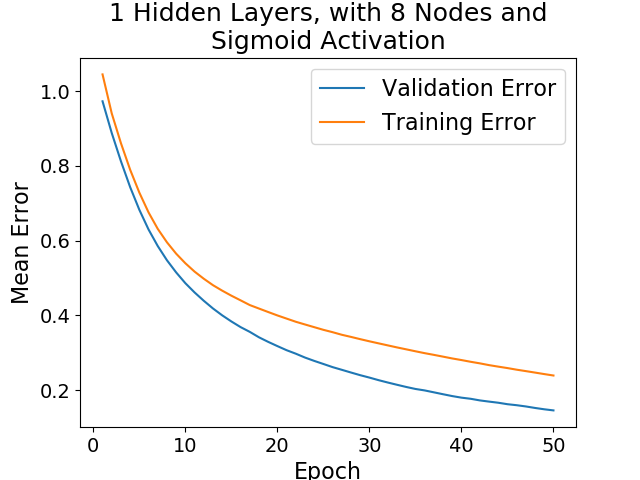
\includegraphics[width=\textwidth]{figs/Iris_Multiclass_Classification_1_Hidden_Layers_with_8_Nodes_and_Sigmoid_Activation.png}
	\end{subfigure}
	%
	\begin{subfigure}[h]{0.23\textwidth}
		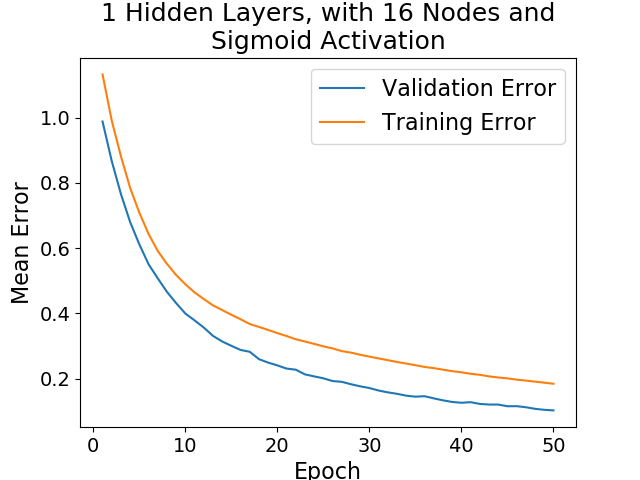
\includegraphics[width=\textwidth]{figs/Iris_Multiclass_Classification_1_Hidden_Layers_with_16_Nodes_and_Sigmoid_Activation.png}
	\end{subfigure}
	%
	\begin{subfigure}[h]{0.23\textwidth}
		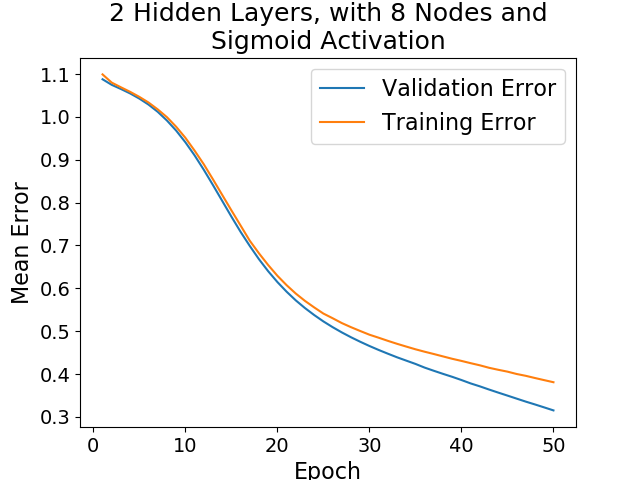
\includegraphics[width=\textwidth]{figs/Iris_Multiclass_Classification_2_Hidden_Layers_with_8_Nodes_and_Sigmoid_Activation.png}
	\end{subfigure}
	%
	\begin{subfigure}[h]{0.23\textwidth}
		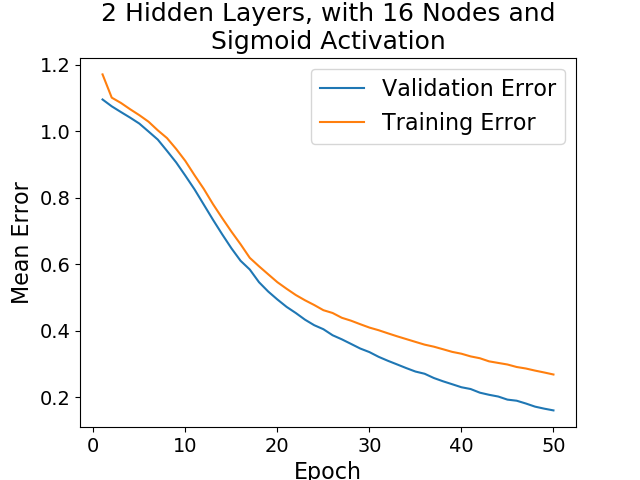
\includegraphics[width=\textwidth]{figs/Iris_Multiclass_Classification_2_Hidden_Layers_with_16_Nodes_and_Sigmoid_Activation.png}
	\end{subfigure}
\end{figure}	
\begin{figure}[h]
	\centering
	\begin{subfigure}[h]{0.23\textwidth}
		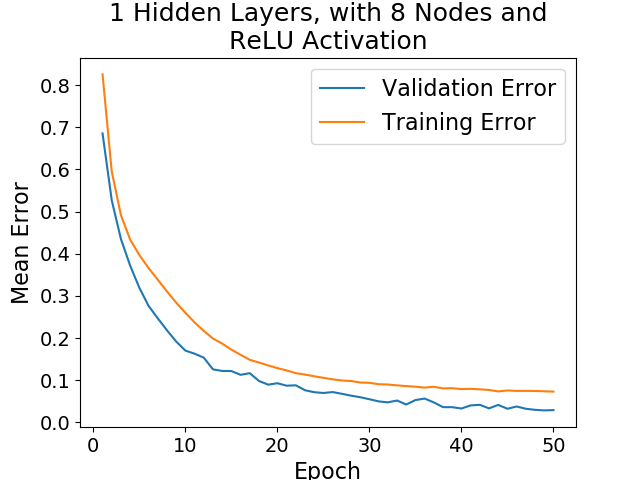
\includegraphics[width=\textwidth]{figs/Iris_Multiclass_Classification_1_Hidden_Layers_with_8_Nodes_and_ReLU_Activation.png}
	\end{subfigure}
	%
	\begin{subfigure}[h]{0.23\textwidth}
		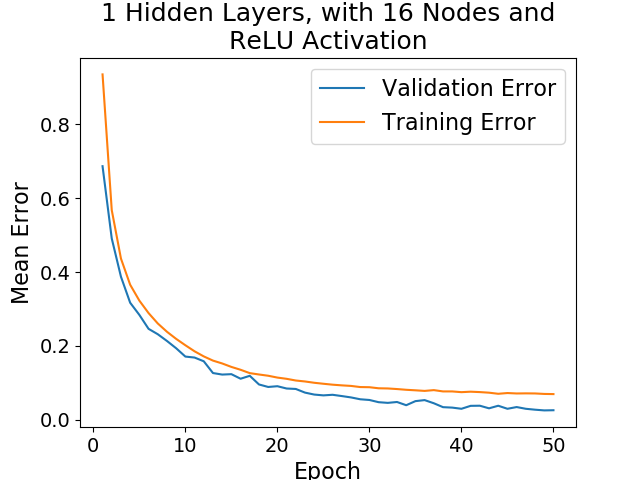
\includegraphics[width=\textwidth]{figs/Iris_Multiclass_Classification_1_Hidden_Layers_with_16_Nodes_and_ReLU_Activation.png}
	\end{subfigure}
	%
	\begin{subfigure}[h]{0.23\textwidth}
		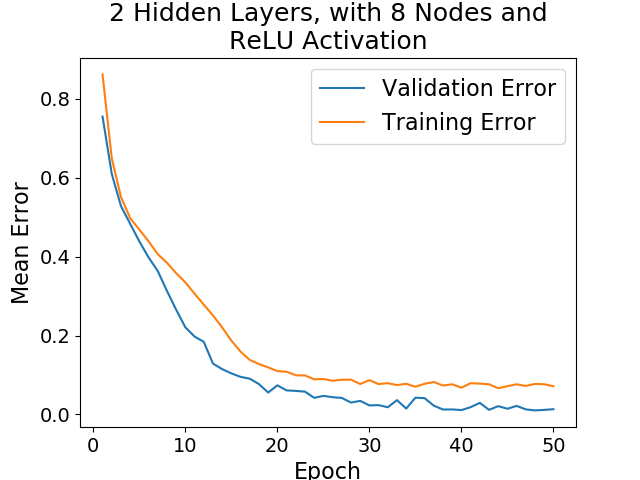
\includegraphics[width=\textwidth]{figs/Iris_Multiclass_Classification_2_Hidden_Layers_with_8_Nodes_and_ReLU_Activation.png}
	\end{subfigure}
	%
	\begin{subfigure}[h]{0.23\textwidth}
		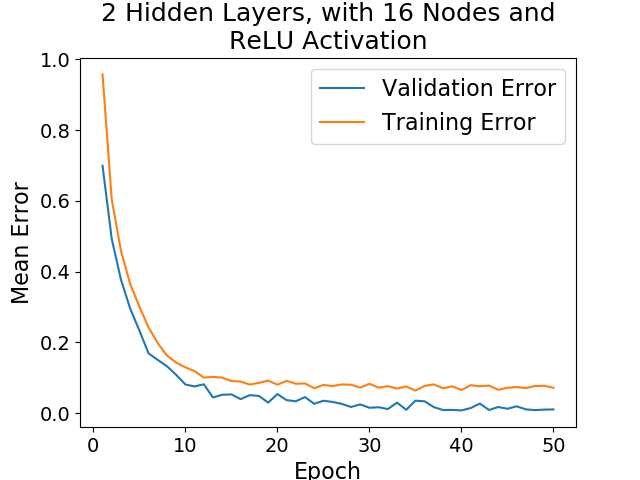
\includegraphics[width=\textwidth]{figs/Iris_Multiclass_Classification_2_Hidden_Layers_with_16_Nodes_and_ReLU_Activation.png}
	\end{subfigure}
\end{figure}	
\begin{figure}[h!]
	\centering
	\begin{subfigure}[h]{0.23\textwidth}
		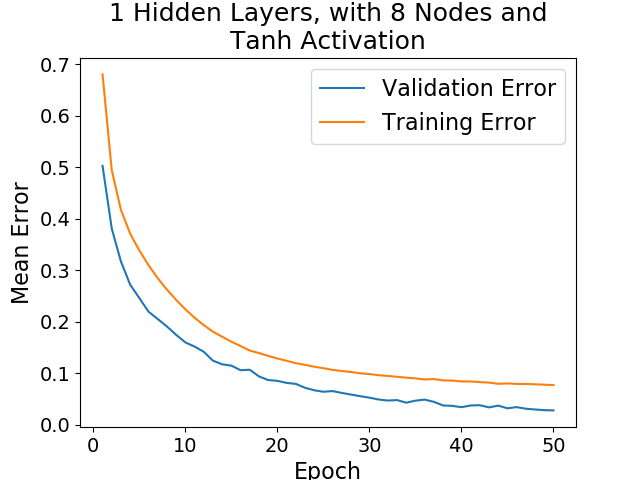
\includegraphics[width=\textwidth]{figs/Iris_Multiclass_Classification_1_Hidden_Layers_with_8_Nodes_and_Tanh_Activation.png}
	\end{subfigure}
	%
	\begin{subfigure}[h]{0.23\textwidth}
		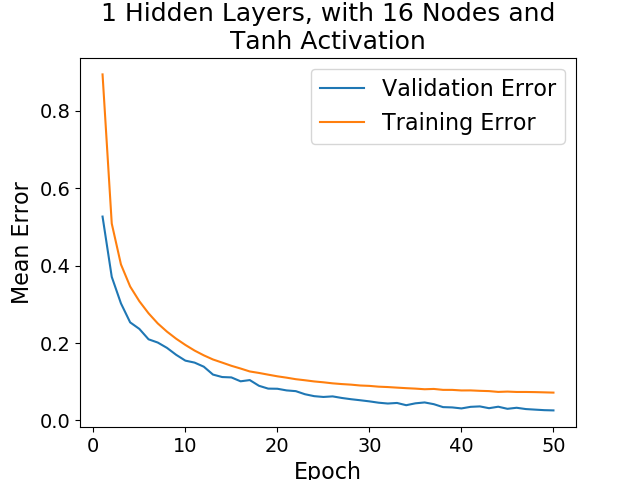
\includegraphics[width=\textwidth]{figs/Iris_Multiclass_Classification_1_Hidden_Layers_with_16_Nodes_and_Tanh_Activation.png}
	\end{subfigure}
	%
	\begin{subfigure}[h]{0.23\textwidth}
		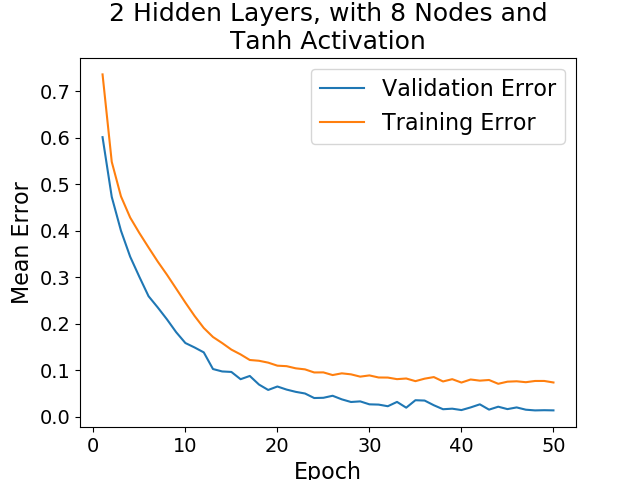
\includegraphics[width=\textwidth]{figs/Iris_Multiclass_Classification_2_Hidden_Layers_with_8_Nodes_and_Tanh_Activation.png}
	\end{subfigure}
	%
	\begin{subfigure}[h]{0.23\textwidth}
		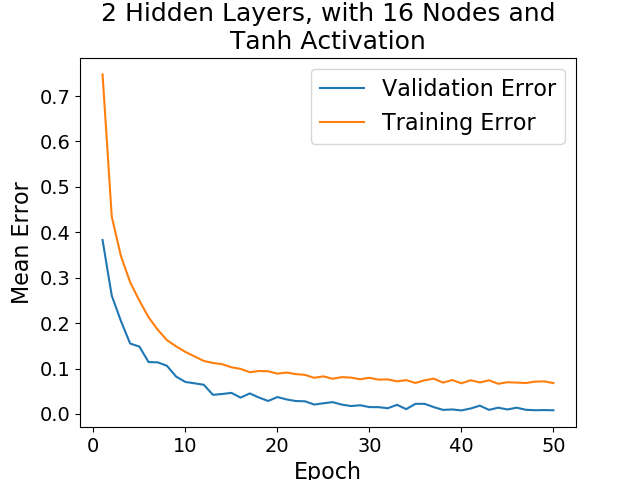
\includegraphics[width=\textwidth]{figs/Iris_Multiclass_Classification_2_Hidden_Layers_with_16_Nodes_and_Tanh_Activation.png}
	\end{subfigure}
\end{figure}
	\setlength{\parindent}{10ex}
	As mentioned in the Data section, this dataset is known to consist of three classes, where two of them are not linearly separable from each other. To visualize this, I once again ran PCA to get the first two primary components, which in total account for 74\% + 22\% = 96\% of the overall variance:
	
		\begin{center}
		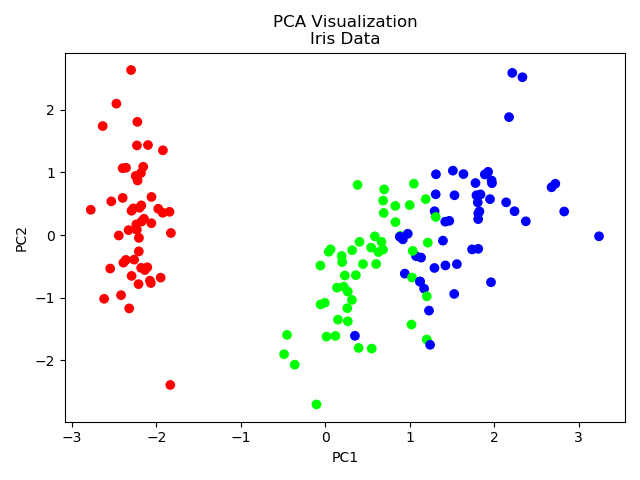
\includegraphics[scale=0.3]{figs/iris_PCA.png}
	\end{center}

We can see that the red-colored class is linearly separable from the green and blue overlap a fair amount. So, although the neural network architectures trained and evaluated in the experiments above did an excellent job classifying all of the test examples, when I ran a quick experiment where I left out the hidden layers, the model did not do as well. This architecture is equivalent to a softmax classifier, where, although the model does work for multiple classes, it still uses only linear boundaries to separate the classes. The trained model resulted in a mean test error of $\approx$ 0.37, and a classification accuracy of $\approx$ 91.7\%. The confusion matrix for the resulting model on the test data is below:
	 		\begin{center}
	 	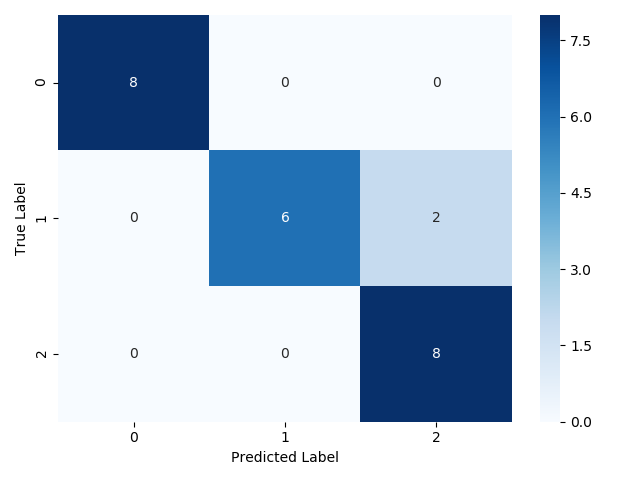
\includegraphics[scale=0.3]{figs/iris_conf.png}
	 \end{center}
 
 We can see that there is some confusion between class \#1 and class \#2 using this model, whereas the non-linear models were able to handle the overlapping data and consistently label the test data correctly. This helps confirm that the multi-layer models are working as expected, and performing better on non-linearly separable data than a linear model. 
 
 As far as comparing the non-linear networks from the experiments in the chart and plots, although all perform well, the models with the sigmoid activation function do seem to be minimizing the error function at a slower rate, evidenced by the less-steep descent the error trajectories in the earlier epochs, as opposed to the steep error drop-offs in the ReLU and tanh trials. The sigmoid trials also have the highest test error. Perhaps, if I were to train the model for a higher number of epochs, the error rate would fall to the same as the other models. Performance of both the ReLU and tanh-based models is as close to equivalent as one could get.
 
 So, again, this is a simple, easy dataset, chosen for the most part to demonstrate the functionality of the system prior to attempting to fit a model to a much more complex dataset. From these three initial experiments, I feel confident that the algorithm has been implemented correctly, and am ready to move on to a more complex experiment.
\end{quote}

\subsubsection*{RAVDESS Speech Emotions Dataset: Multiclass Classification}
\begin{quote}
	\setlength{\parindent}{10ex}
	\quad\quad\quad\quad As described in the Data section, this experiment involved a much more complex dataset, which I chose because of my interest in speech signal processing, and automatic speech recognition in general. To describe a bit more about the feature-selection process, I was initially planning to train the model on MFCC features for individual frames, but quickly realized that this would not be an ideal feature set to use due to the high variation in/dynamic nature of vocal formants across a sentence-length utterance. So instead of training on frame-level features, I averaged all of the MFCC values across the entire utterance, in hopes that it would capture the overall intensity and formant frequencies inherent to an utterance belonging to a particular emotion being conveyed. 
	
	I hate to give away the punchline, but I want to begin by saying that despite all of my efforts, I was not able to achieve high accuracy on this dataset. I do think that it may be due to the choice of features, and also due to the fact that I did not classify based on gender, that is, the ``angry" class contains examples produced by both male and female speakers. Formant frequencies certainly differ across genders, particularly F0 (which affects all other formants), and this may have added noise to the dataset that hindered the ability for the model to reliably predict the correct label. I also noticed, after perusing some other's approaches on Kaggle, that a DNN may not be the best approach to modeling this type of dataset (typically, a CNN is used, with a different set of features). Because there are so many dynamic features present in speech, which certainly can be related to the emotion being conveyed in the utterance, a model that cannot account for dynamic attributes of the input is not ideal. 
	
	We can also visualize the data using PCA to get a better sense of the variance between the class distributions, note, in this case PC1 accounted for 56\% of the overall variance, and PC2 for 8\%:
		 		\begin{center}
		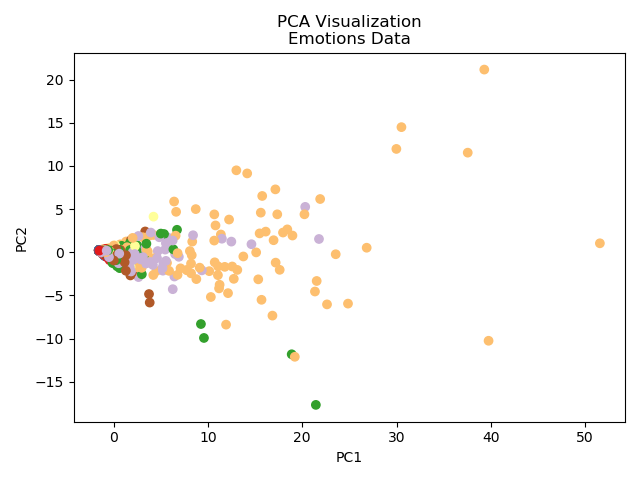
\includegraphics[scale=0.3]{figs/PCA_emotions.png}
	\end{center}
	
	As we can see, there is quite a bit of overlap in these classes, so I do not have high hopes that we will achieve high accuracy...however, we should still be able to train a network to perform better than chance, considering we can incorporate non-linearities that can deal with non-linearly separable data. After all that has been said, in spire of the challenges, I'd still like to document the experiments that I performed in an effort to achieve a respectable classification accuracy on this dataset.
	
	Although I began by using the same parameter search as in the preceding experiments, I quickly saw that this model would require a more comprehensive parameter search. In the early experiments, I was seeing accuracies as low as chance, which for an eight-class dataset is 12.5\%. So, I decided to perform a more comprehensive hyperparameter search, in which I trained a number of models in order to identify which architecture and activation function would result in the best performing model. The parameters over which I searched during this step were:
	
	\begin{itemize}
		\item [] Number of layers: [1, 2, 3, 4, 5, 10, 20, 25]
		\item [] Hidden layer activation: [sigmoid, tanh, relu]
		\item [] Nodes per layer: [16, 24, 36, 48]
		\item [] Learning rates: [0.1, 0.01, 0.005, 0.001]
	\end{itemize}

	As described in the discussion of weights in the methods section, when I realized that training a model on this dataset would be tricky, I did some research on the ideal way to initialize weights, and found the methods listed in that section. Although I did not use those methods for the previous three experiments, I did use them for the hyperparameter search, in hopes that they would improve the gradient descent process and result in better error rates. In hopes of achieving better performance, I also decided to use the early stopping regularization technique, setting the model to stop after three epochs with increasing validation error. I let the model train for up to 500 epochs (I was a bit desperate...), but it seldom went even close to that many epochs.
	
	The best model architecture (in terms of accuracy) identified during this hyperparameter search was a model with five hidden layers, 36 nodes each, ReLU activation, and a 0.01 learning rate. The model's accuracy on the test data was $\approx$ 40.4\%, which doesn't seem terribly good at first glance, but considering that we are dealing with eight classes, and chance is 12.5\%, this is not completely abysmal. Now that we are working with a more complex dataset, I'm not surprised that the ReLU activation function is resulting in the best performance, as it is known for not only converging quickly, but also for imparting sparsity to a model, meaning that not all neurons are activated at once. This occurs because any time the ReLU function is applied to a negative input, it outputs zero, essentially meaning that the neuron in question is not activated. For a complex model, this is a positive feature, as it limits overfitting (see citation \#4 for source). Now, we can take a look at a confusion matrix to get a better sense of what the model is struggling with:
	
	\begin{center}
		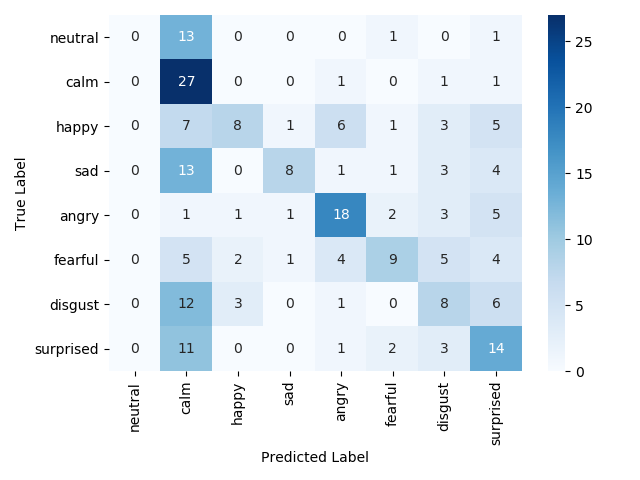
\includegraphics[scale=0.5]{figs/Emotions_Initial_Best_Conf.png}
	\end{center}
	
	It appears that the model has a tendency to incorrectly predict the label `calm' for a very high number of test examples. In fact, almost all of the `neutral' examples are predicted to be `calm'. Simply thinking about this from an auditory/perceptual point of view, it makes sense, one who is speaking calmly tends to also be speaking in a neutral tone. It also makes sense that `calm' would be a decent default guess if the particular emotion conveyed is not very strong, thus difficult to categorize. Since the features selected to train this model are pulled directly from the speech signal, specifically the intensity levels of binned frequencies using the mel-scale, which was designed to emulate human perception, it follows that the model would be making similar confusions to those that a human may make. Again, by flattening these features into a single vector for the entire utterance, any dynamic information present in the sound is eliminated, which is certainly necessary for conveying tone/emotion, so the relatively poor performance is not surprising.
	
	I do, however, want to include the training and validation error trajectories, as they show some rather strange behavior:
	
		\begin{center}
		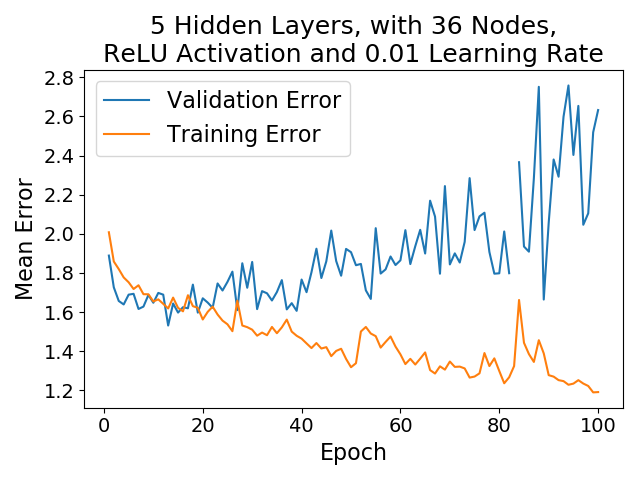
\includegraphics[scale=0.4]{figs/Emotions_Initial_Best_Cost.png}
	\end{center}

	We can see here that while the training error does trend downward (with some noise, as we are descending using stochastic gradient descent thus the gradient is not consistent across epochs), the validation error is very erratic, trending upwards. However, it was not until the 100th epoch that the validation error rose for three epochs in a row, thus the model continued to run until that point, fitting to the training data. This behavior is indicative of the model having low bias and high variance, a sign of overfitting. However, this evidence of overfitting in conjunction with the relatively decent accuracy, made me wonder if perhaps the validation set may not fully reflect the training/testing data. This could be because there are both male and female speakers, so perhaps the validation set has a disproportional amount of one gender, whereas the other sets do not. I will attempt to address this issue later in the analysis!
	
	I won't include the results of every single model searched (after all, this was a search over 384 different models), but there are a few interesting observations worth mentioning. Over the entire search of 384 different architectures/hyperparameter settings, there were 72 models with final test accuracies of 35\% or above, which I considered successful given the fairly significant performance above chance. Several details regarding these top-performing models are in the tables below:
	
\begin{table}[h]
	\centering
	\begin{tabular}{|r|c|c|c|c|c|}
		\hline
		& \# & \begin{tabular}[c]{@{}c@{}}Average\\ Accuracy\end{tabular} & \begin{tabular}[c]{@{}c@{}}Average\\ Error\end{tabular} & \begin{tabular}[c]{@{}c@{}}Mode\\ Hidden\\ Layers\end{tabular} & \begin{tabular}[c]{@{}c@{}}Mode\\ Nodes\end{tabular} \\ \hline
		ReLU    & 24 & 36.84                                                      & 2.07                                                    & 3                                                              & 36                                                   \\ \hline
		Sigmoid & 11 & 36.56                                                      & 1.79                                                    & 2                                                              & 12                                                   \\ \hline
		Tanh    & 37 & 36.66                                                      & 1.77                                                    & 4                                                              & 48                                                   \\ \hline
		Total   & 72 & 36.71                                                      & 1.88                                                    & 2                                                              & 48                                                   \\ \hline
	\end{tabular}
\end{table}

We can see that of the best performing models, the majority had tanh as the nonlinear activation for the hidden layers, followed by ReLU, with sigmoid trailing behind. However, the successful models using the ReLU function resulted in the best average accuracy, but only by a slight fraction. Oddly, the average error for the successful ReLU-based models was a fair bit higher than that of both of the other activation functions, despite similar accuracies. 

I also took a look at the most successful learning rates, and found that there were few successful models with the largest learning rate (0.1), a total of seven, six of which were sigmoid-based. Since the sigmoid activation function is associated with slower convergence, it makes sense that models based on this activation function performed best when descending along the gradient with larger steps. The remaining successful models were fairly balanced in terms of learning rates, and within each set corresponding to each learning rate, they were balanced in terms of activation function. At a glance, however, it seems like the successful models with smaller learning rates were associated with more complexity in terms of hidden layer depth as well as number of nodes per layer. This may be because the more complex models have a similarly more complex cost function to minimize, thus smaller nudges against the gradient may prevent overfitting, resulting in better generalization.  Similarly, the smaller the learning rate, the less dramatic the oscillations present in the per-epoch errors, particularly in the case of the validation error, unlike the plot above for the best performing model. One such example is below:

\begin{figure}[h!]
	\centering
	\begin{subfigure}[h]{0.23\textwidth}
		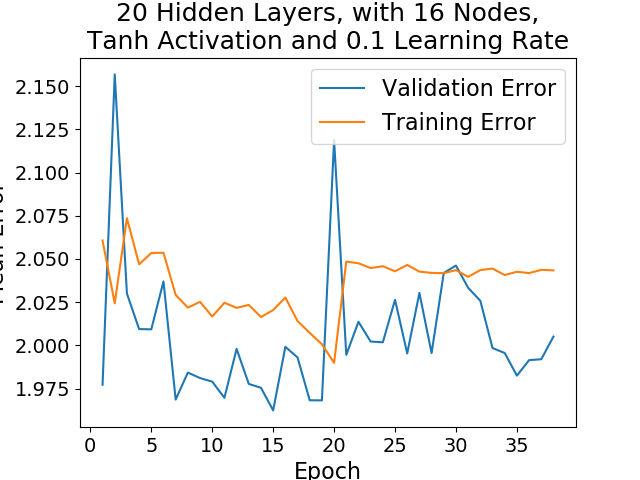
\includegraphics[width=\textwidth]{figs/Emotions_Multiclass_Classification_20_Hidden_Layers_with_16_Nodes_Tanh_Activation_and_0.1_Learning_Rate.png}
	\end{subfigure}
	%
	\begin{subfigure}[h]{0.23\textwidth}
		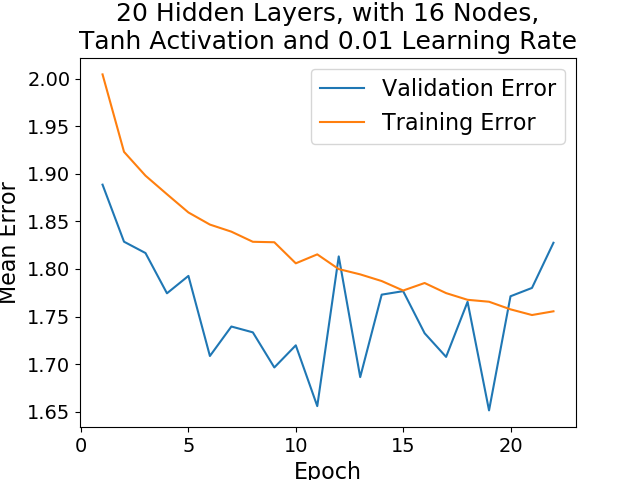
\includegraphics[width=\textwidth]{figs/Emotions_Multiclass_Classification_20_Hidden_Layers_with_16_Nodes_Tanh_Activation_and_0.01_Learning_Rate.png}
	\end{subfigure}
	%
	\begin{subfigure}[h]{0.23\textwidth}
		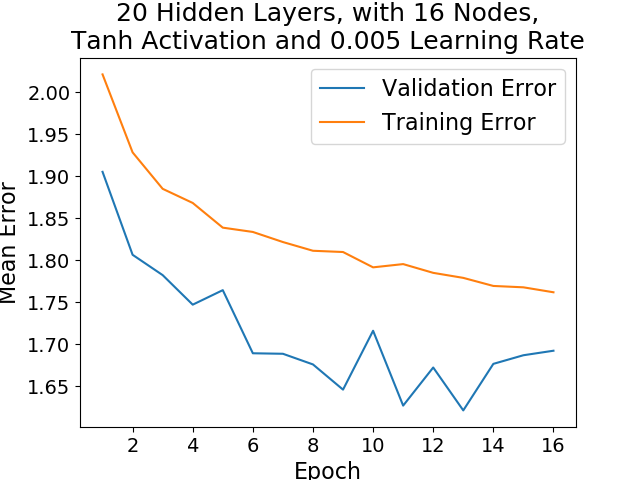
\includegraphics[width=\textwidth]{figs/Emotions_Multiclass_Classification_20_Hidden_Layers_with_16_Nodes_Tanh_Activation_and_0.005_Learning_Rate.png}
	\end{subfigure}
	%
	\begin{subfigure}[h]{0.23\textwidth}
		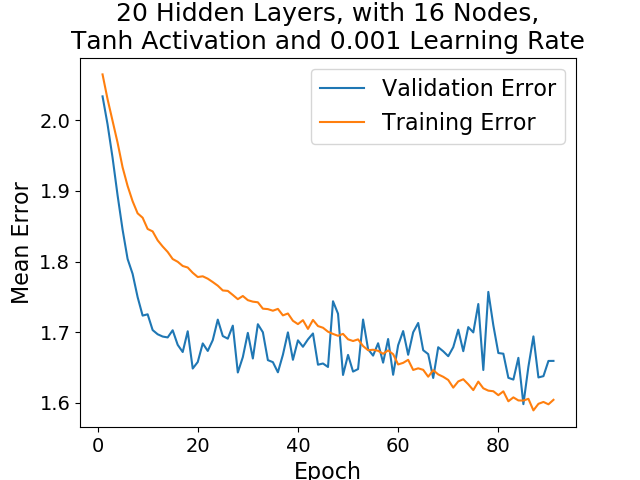
\includegraphics[width=\textwidth]{figs/Emotions_Multiclass_Classification_20_Hidden_Layers_with_16_Nodes_Tanh_Activation_and_0.001_Learning_Rate.png}
	\end{subfigure}
\end{figure}

 In turn, the very complex models simply do not perform well with large learning rates, as evidenced by the following per-epoch train-validate error plot, in which it appears that the model got stuck in a non-ideal position in the cost function:

\begin{center}
	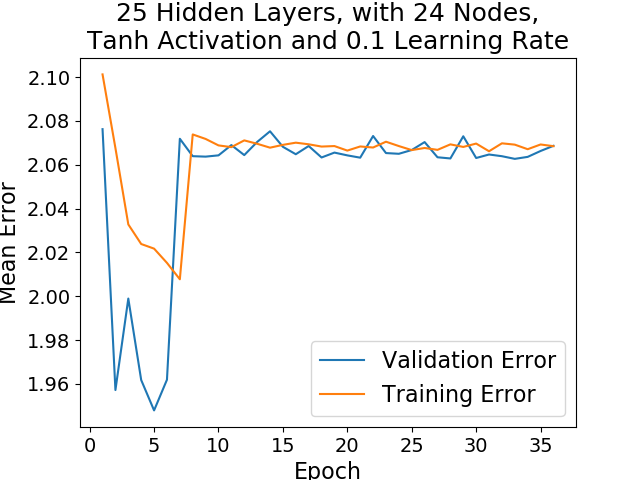
\includegraphics[scale=0.5]{figs/Emotions_Multiclass_Classification_25_Hidden_Layers_with_24_Nodes_Tanh_Activation_and_0.1_Learning_Rate.png}
\end{center}


Now, In an attempt to improve model performance, I wanted to do one more experiment with this dataset. I did a bit of scrounging around online to get some ideas on how to improve the model, as this is a fairly commonly used dataset. I knew I wanted to investigate the aforementioned issue with folding male and female speakers into the same classes, and I came across an example where the person experimenting with the dataset split the classes into male and female to train the model (so there would be two times as many classes, two per emotion), then folded the classes back into single emotions to evaluate the model on the test data (see citation \#5). Inspired by this approach, I performed a similar experiment, splitting the classes prior to training. I decided to only train the best twenty of the models described above (in terms of highest accuracy), as I would anticipate these would also perform best on the modified dataset. I was also curious whether changing the early stopping criteria would improve performance, so I evaluated the models using a patience of 2, 3, and 4, that is, training would conclude after 2, 3, or 4 epochs with increasing validation error. For the sake of space, I will not give details for every model evaluated in this experiment, but will simply provide details for the best performing model for each early stopping setting, and a short analysis of the overall results for the best model.

\begin{table}[h]
	\centering
	\begin{tabular}{|c|c|c|c|c|c|c|c|}
		\hline
		\begin{tabular}[c]{@{}c@{}}Early\\ Stopping\\ Patience\end{tabular} & \begin{tabular}[c]{@{}c@{}}Activation\\ Function\end{tabular} & \begin{tabular}[c]{@{}c@{}}Hidden\\ Layers\end{tabular} & \begin{tabular}[c]{@{}c@{}}Nodes\\ Per\\ Layer\end{tabular} & \begin{tabular}[c]{@{}c@{}}Learning\\ Rate\end{tabular} & \begin{tabular}[c]{@{}c@{}}Raw \\ Error\end{tabular} & \begin{tabular}[c]{@{}c@{}}Raw\\ Accuracy\\ (16 classes)\end{tabular} & \begin{tabular}[c]{@{}c@{}}Folded\\ Accuracy\\ (8 classes)\end{tabular} \\ \hline
		2                                                                   & Tanh                                                          & 10                                                      & 36                                                          & 0.001                                                   & 2.09                                                 & 33.3\%                                                                & 40.35\%                                                                 \\ \hline
		3                                                                   & Tanh                                                          & 1                                                       & 24                                                          & 0.005                                                   & 1.86                                                 & 38.16\%                                                               & 43.86\%                                                                 \\ \hline
		4                                                                   & ReLU                                                          & 4                                                       & 48                                                          & 0.005                                                   & 2.38                                                 & 39.04\%                                                               & 43.43\%                                                                 \\ \hline
	\end{tabular}
\end{table}
	
	We can see that we do get a slight increase in accuracy when we train on the data broken out by gender, and then fold the data back into the eight emotion-based classes, although the gain is only approximately 3.5\% (40.4\% versus 43.86\%). Interestingly, the best performing model in this case is the simplest -- a model with tanh activations, only one hidden layer, and 24 nodes per layer. The final raw (16 class) and folded (8 class) confusion matrices for the best performing model are below:
	
	\begin{figure}[h!]
		\centering
		\begin{subfigure}[h]{0.45\textwidth}
			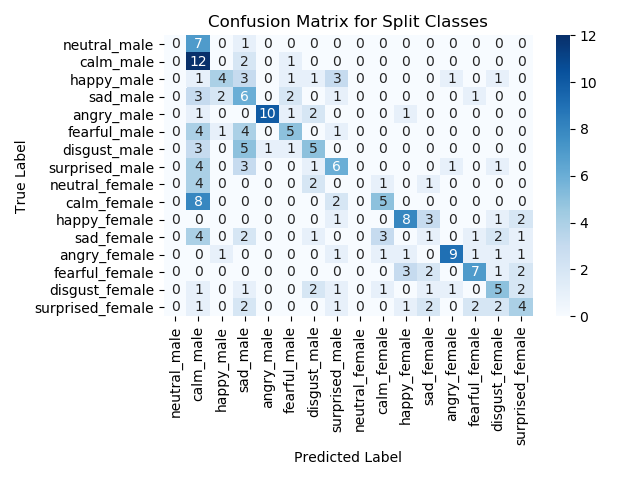
\includegraphics[width=\textwidth]{figs/final_conf_raw.png}
		\end{subfigure}
		%
		\begin{subfigure}[h]{0.45\textwidth}
			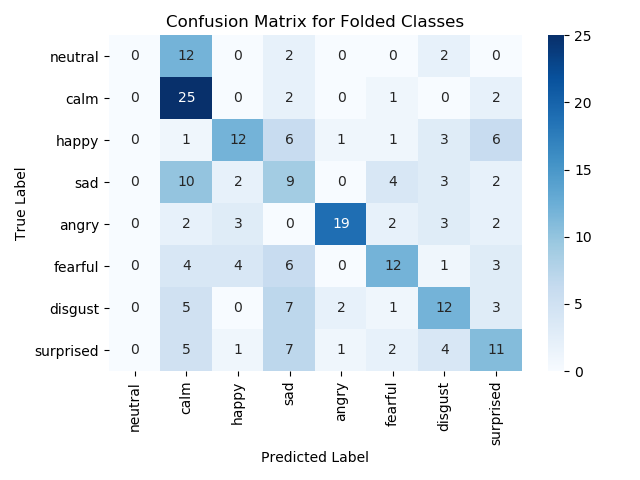
\includegraphics[width=\textwidth]{figs/final_conf_folded.png}
		\end{subfigure}
	\end{figure}

Taking a quick look at the train/validate trajectory for this model, it does look as though it is very well-behaved as it minimizes the error:

\begin{center}
	\includegraphics[scale=0.35]{figs/final_analysis_best.png}
\end{center}

Although there are certainly other analyses that could be done (I'd love to take a look at the actual gradient size during training, to explicitly check for the vanishing/exploding issues, as well as determine whether the ReLU function was resulting in any dead nodes), my report is already quite long, so I will stop here. I'm fairly pleased with the final best accuracy I achieved on this tricky dataset, despite it being relatively far from 100\%. I'd be curious to find out how well humans perform at categorizing the utterances, as I'm doubtful that we ourselves could achieve higher than $\approx$ 60-70\% accuracy on such a task. Regardless, this was a very interesting experiment, and I enjoyed the process significantly!
	
	
\end{quote} 

\subsection*{Discussion and Conclusions}
\begin{quote}
\setlength{\parindent}{10ex}
\quad\quad\quad\quad After all of that time spent on implementing the neural network frameworks, and the associated experiments, I'm glad to say that I'm feeling quite a bit more knowledgeable about the overall process, including backpropagation. It's no longer a mysterious pile of symbols, although it is still pretty magical, in spite of just being, essentially, a series of linear algebra and calculus operations. However, there are a number of aspects of neural networks that I wish I'd had more time to wrap my mind around, as I do think they would have provided additional insight into the behaviors observed in the experiments.

One of these aspects is to more fully understand how the overall cost function is affected by the choice of hidden layer activation functions. There is a lot of information on the web about which functions are ``better", but little explanation of exactly why. I still feel a bit like I am groping around in the dark when I discuss why certain activation functions result in better performance, and am still not certain about how to make an educated guess as to what hidden layer activation functions would be better for certain problems. There must be a methodical way to make this choice besides simply searching various architectures, but at this point in my studies, I'm not sure what that method is. As mentioned in the final experiment, I would also like to take a closer look at the gradient size during training, and do wish I would have had time to do that in this project. In retrospect, I could have picked a better-behaved dataset for the final experiment, and perhaps would have had more time to investigate these issues instead of trying to improve the model accuracy in other ways. Perhaps this will be a future project.

I would also have liked to have included in my implementation an option for batch and mini-batch training. I would have liked to have seen how the results for the RAVDESS dataset may have differed using the alternate training techniques. I may still implement these for my own interest over the summer, as mentioned earlier, it shouldn't be hard at all to accumulate the weights and apply them at once at the end of a (mini-)batch. I also would have liked to have spent a bit more time considering the efficiency of my implementation -- for anything larger than ~20 layers, it is pretty slow. I know there are way to speed up the process, but implementing it in the way that I did was useful for becoming more familiar with the algorithm.

I also really would have liked to try a bagging or boosting approach to improve performance on the emotions dataset. Since I noticed some evidence for high variance/overfitting in the best performing models, and ensemble methods are designed to decrease the variance of the individual models, I think this approach would have helped improve performance at least a bit.

Generally speaking, although I do feel pretty comfortable with the general backpropagation algorithm and mathematics, there is still a \textit{lot} to learn about neural network model training and optimization. I really enjoyed this project and topic, I plan to continue my machine learning journey though my own research over the summer, and in future coursework!
\end{quote}

\subsection*{Citations}
$^1$ https://towardsdatascience.com/weight-initialization-in-neural-networks-a-journey-from-the-basics-to-kaiming-954fb9b47c79

$^2$ http://neuralnetworksanddeeplearning.com/chap2.html

$^3$ https://medium.com/@snaily16/what-why-and-which-activation-functions-b2bf748c0441

$^4$ https://medium.com/@danqing/a-practical-guide-to-relu-b83ca804f1f7

$^5$ https://www.kaggle.com/ejlok1/audio-emotion-part-3-baseline-model

$^6$ https://smartlaboratory.org/ravdess/
\end{document}

